% ---------------------------------------------------------------------------- %
\subsection{Wichtige Daten}
\label{subsec:daten}
% ---------------------------------------------------------------------------- %

\begin{table}[h!]
    \centering
    \small
    \caption{Charakteristische R\"ontgenlinien der Anodenmaterialien. \emph{Quelle:} Anhang der Versuchsanleitung}
    \label{tab:anodeSpetralLines}
    \begin{tabular}{lrrrr}
        \toprule

        Material            &
        $\lambda-K\alpha_1$ &
        $\lambda-K\alpha_2$ &
        $\lambda-K\alpha$   &
        $\lambda-K\beta$    \\

        \midrule

        Fe (Z = 26)              &
        \SI{194.00}{\pico\meter} &
        \SI{193.60}{\pico\meter} &
        \SI{193.80}{\pico\meter} &
        \SI{175.66}{\pico\meter} \\

        Cu (Z = 29)               &
        \SI{154.05}{\pico\meter}  &
        \SI{154.44}{\pico\meter}  &
        \SI{154.245}{\pico\meter} &
        \SI{193.23}{\pico\meter}  \\

        Mo (Z = 42)              &
        \SI{70.93}{\pico\meter}  &
        \SI{71.36}{\pico\meter}  &
        \SI{71.145}{\pico\meter} &
        \SI{63.26}{\pico\meter}  \\

        \bottomrule
    \end{tabular}
\end{table}

Tabelle \ref{tab:anodeSpetralLines} enth\"alt die Daten der charakteristischen
Spektrallinien  der Anodenmaterialien  (zu finden  in der  Veruchsanleitung im
Anhang).  Da die beiden $\alpha$-Linien sehr nahe beieinander liegen und daher
beinahe immer als  lediglich ein Peak zu sehen sind,  wurde ein arithmetischer
Mittelwert $K\alpha$ bestimmt,  welcher in den folgenden  Rechnungen und Plots
jeweils benutzt wird (z.B. f\"ur die Bragg'sche Gleichung).

% ---------------------------------------------------------------------------- %
\subsection{Versuch 3.1 -- Spektra der R\"ohren, Analyse von LiF}
\label{subsec:spektra}
% ---------------------------------------------------------------------------- %

Als Erstes wurden die Spektra der drei R\"ohren (Kupfer, Eisen, Molybd\"an) mit
einem LiF-Kristall bei \SI{35}{\kilo\volt} aufgenommen.

\begin{figure}[h!]
    \centering
    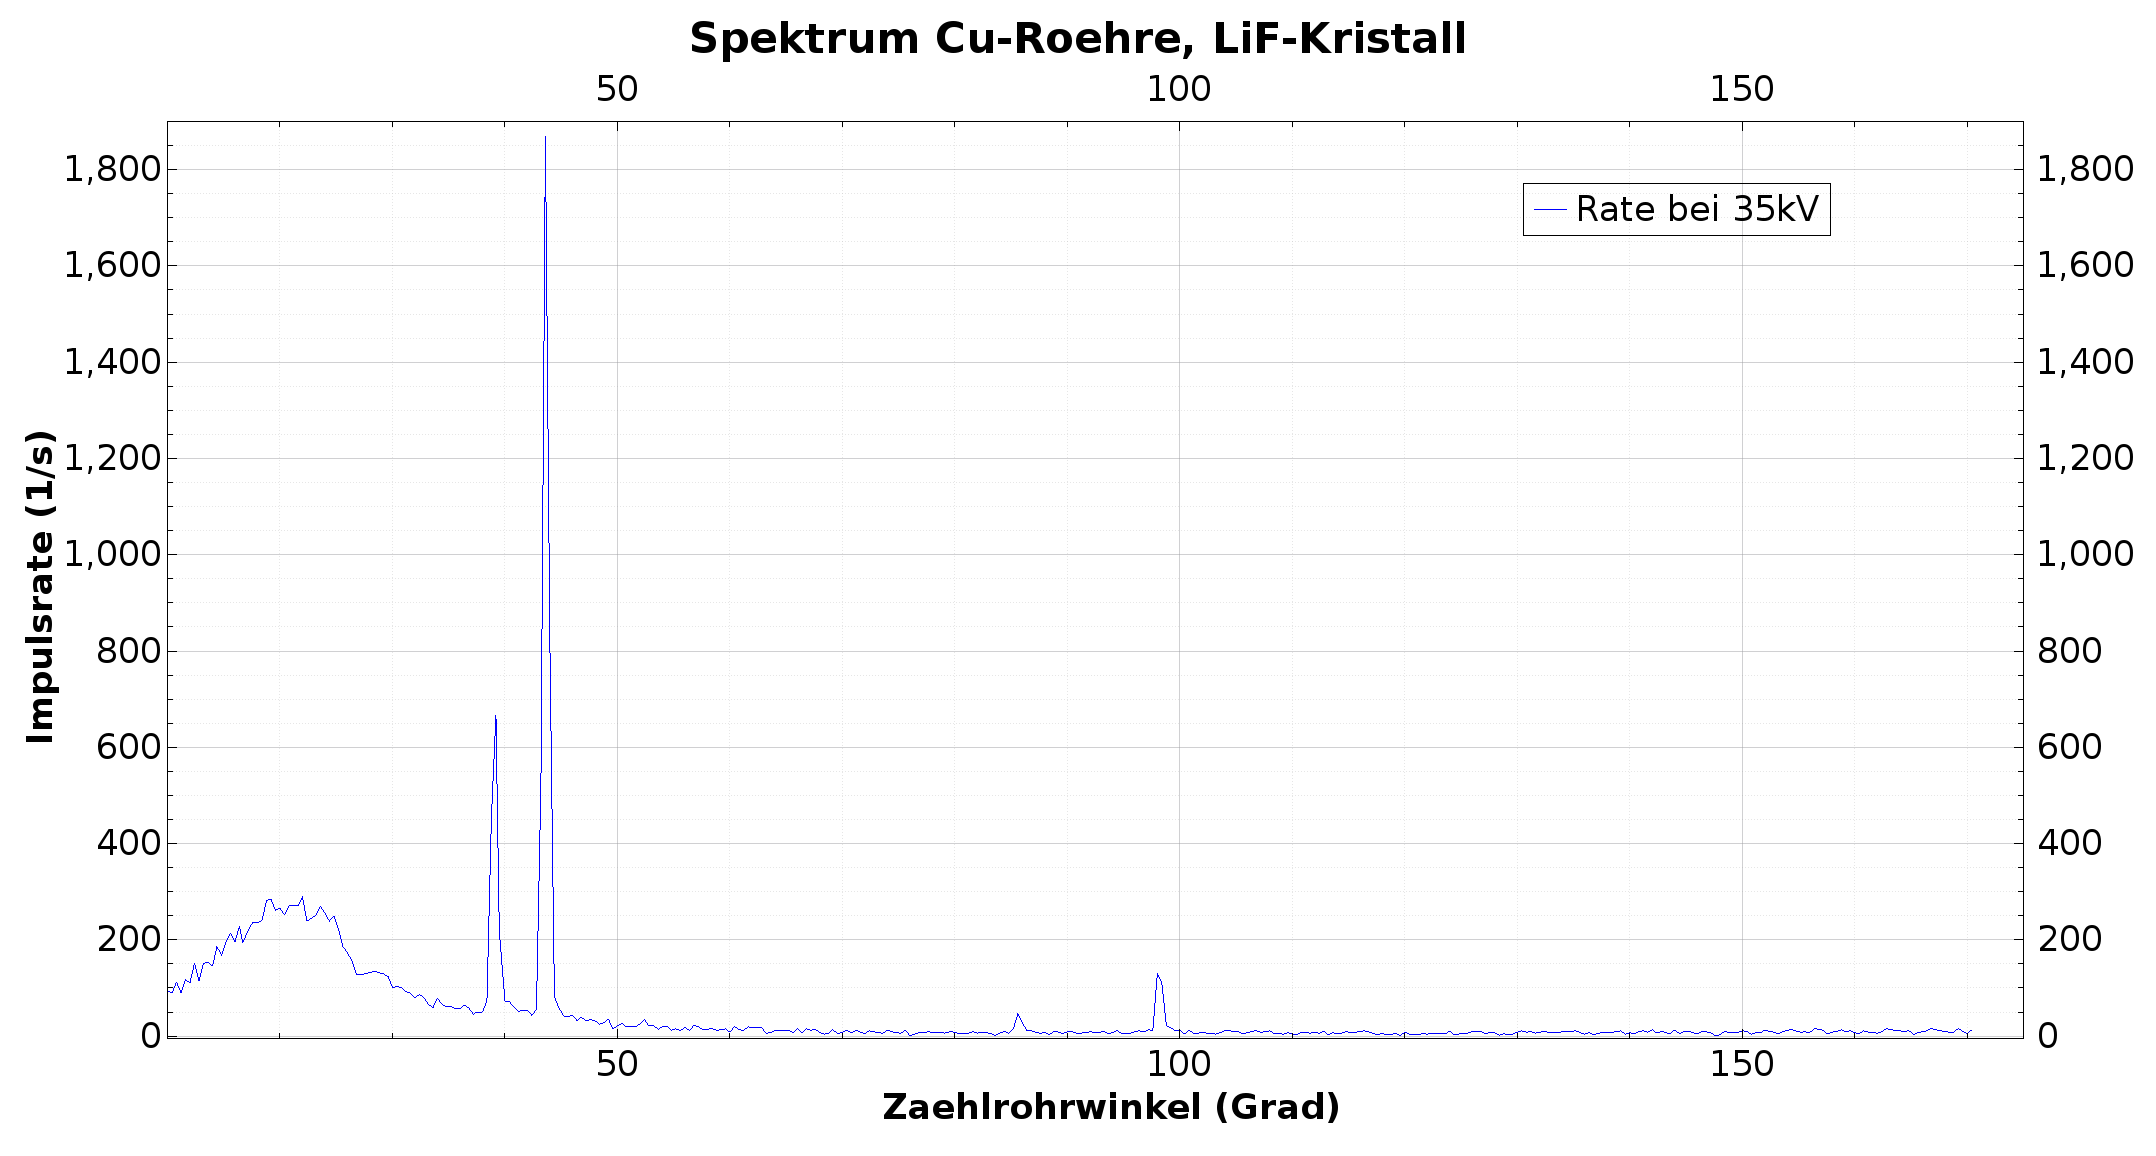
\includegraphics[width=\textwidth]{images/31_1_spektrum-Cu.png}
    \caption{Spektrum mit Kupferr\"ohre}
    \label{fig:spektrum:cu}
\end{figure}

\begin{figure}[h!]
    \centering
    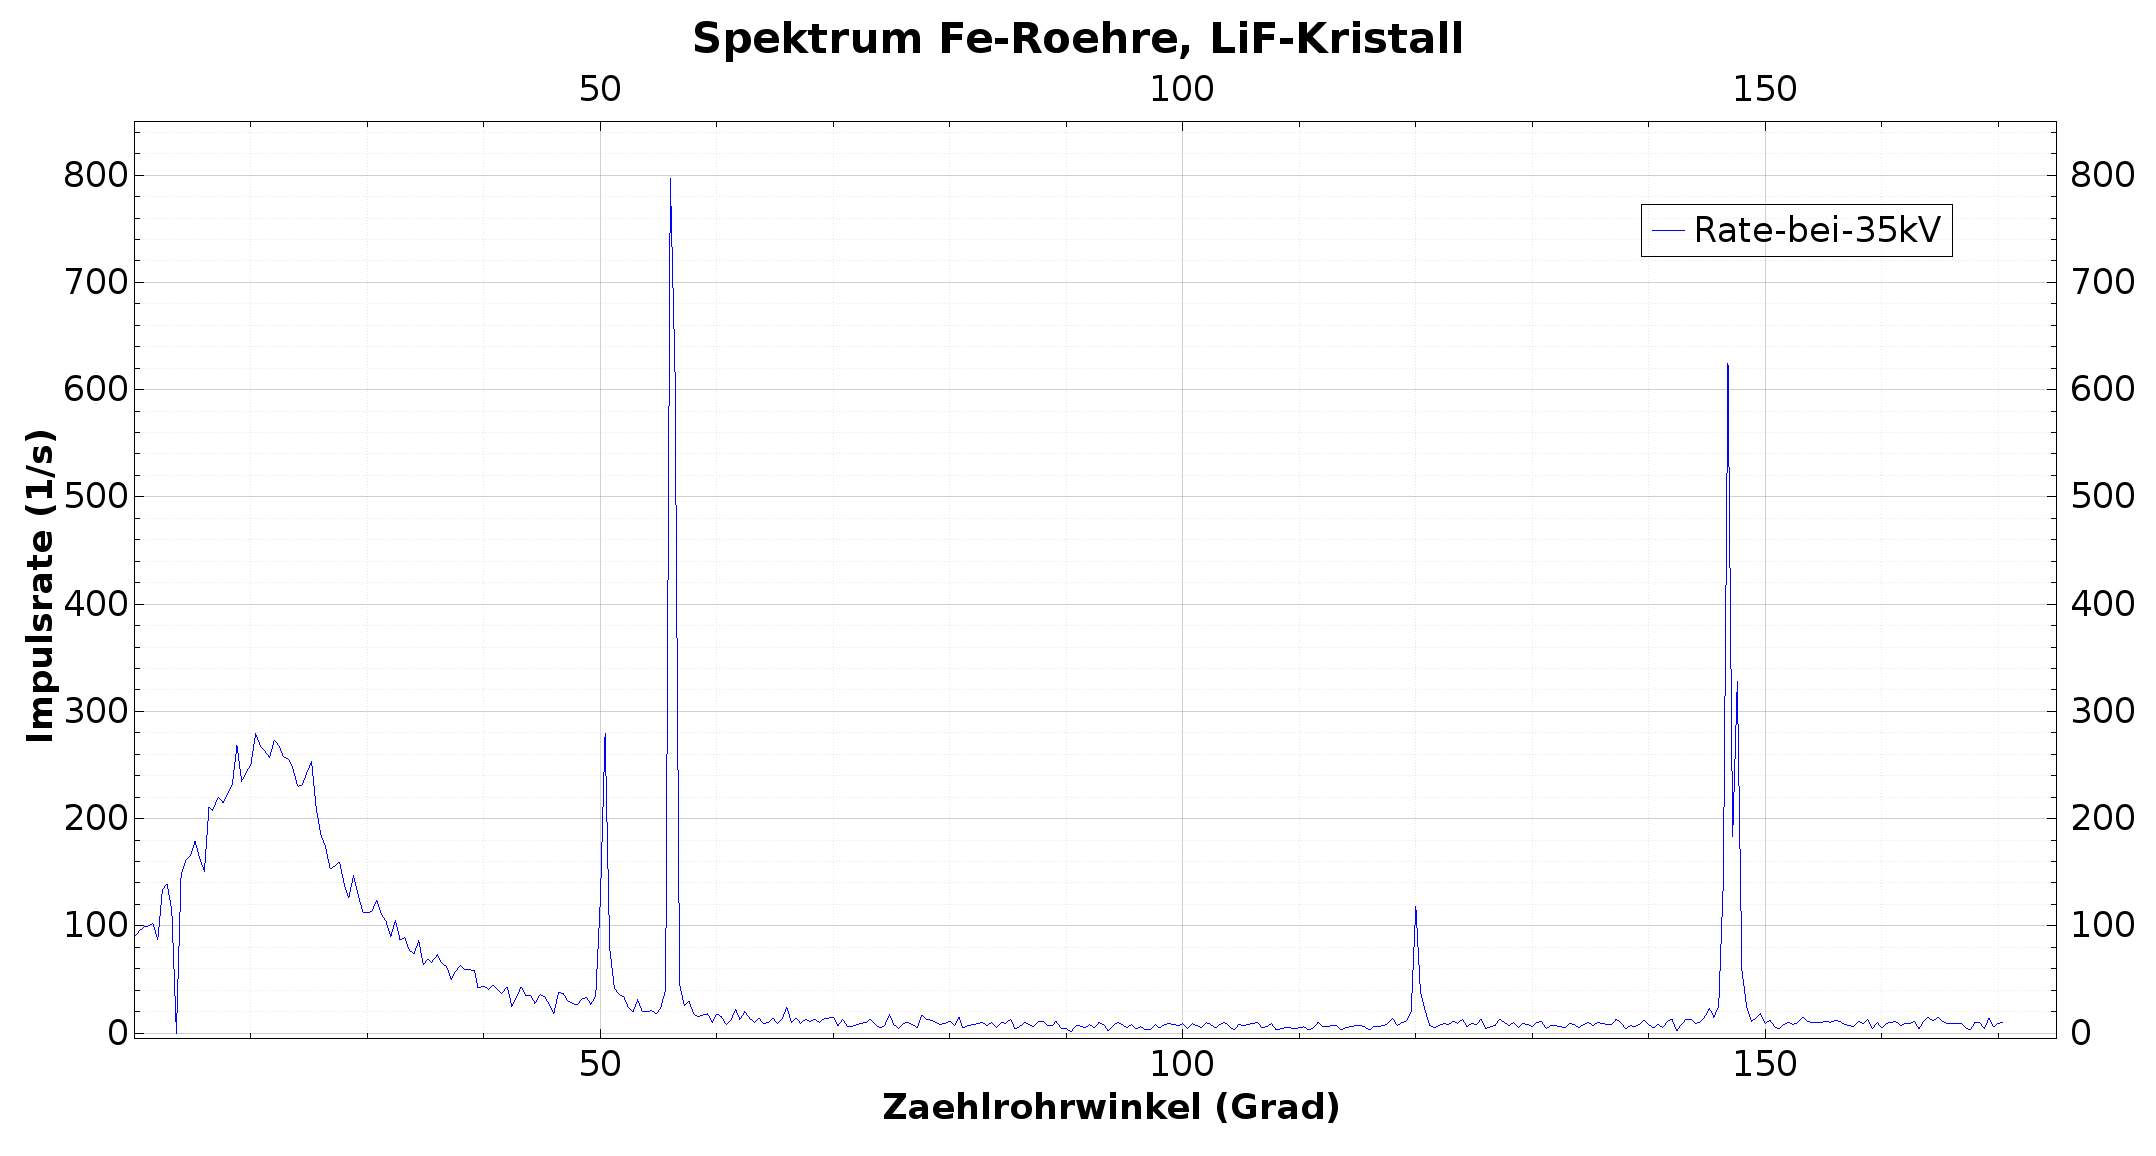
\includegraphics[width=\textwidth]{images/31_2_spektrum-Fe.png}
    \caption{Spektrum mit Eisenr\"ohre}
    \label{fig:spektrum:fe}
\end{figure}

\begin{figure}[h!]
    \centering
    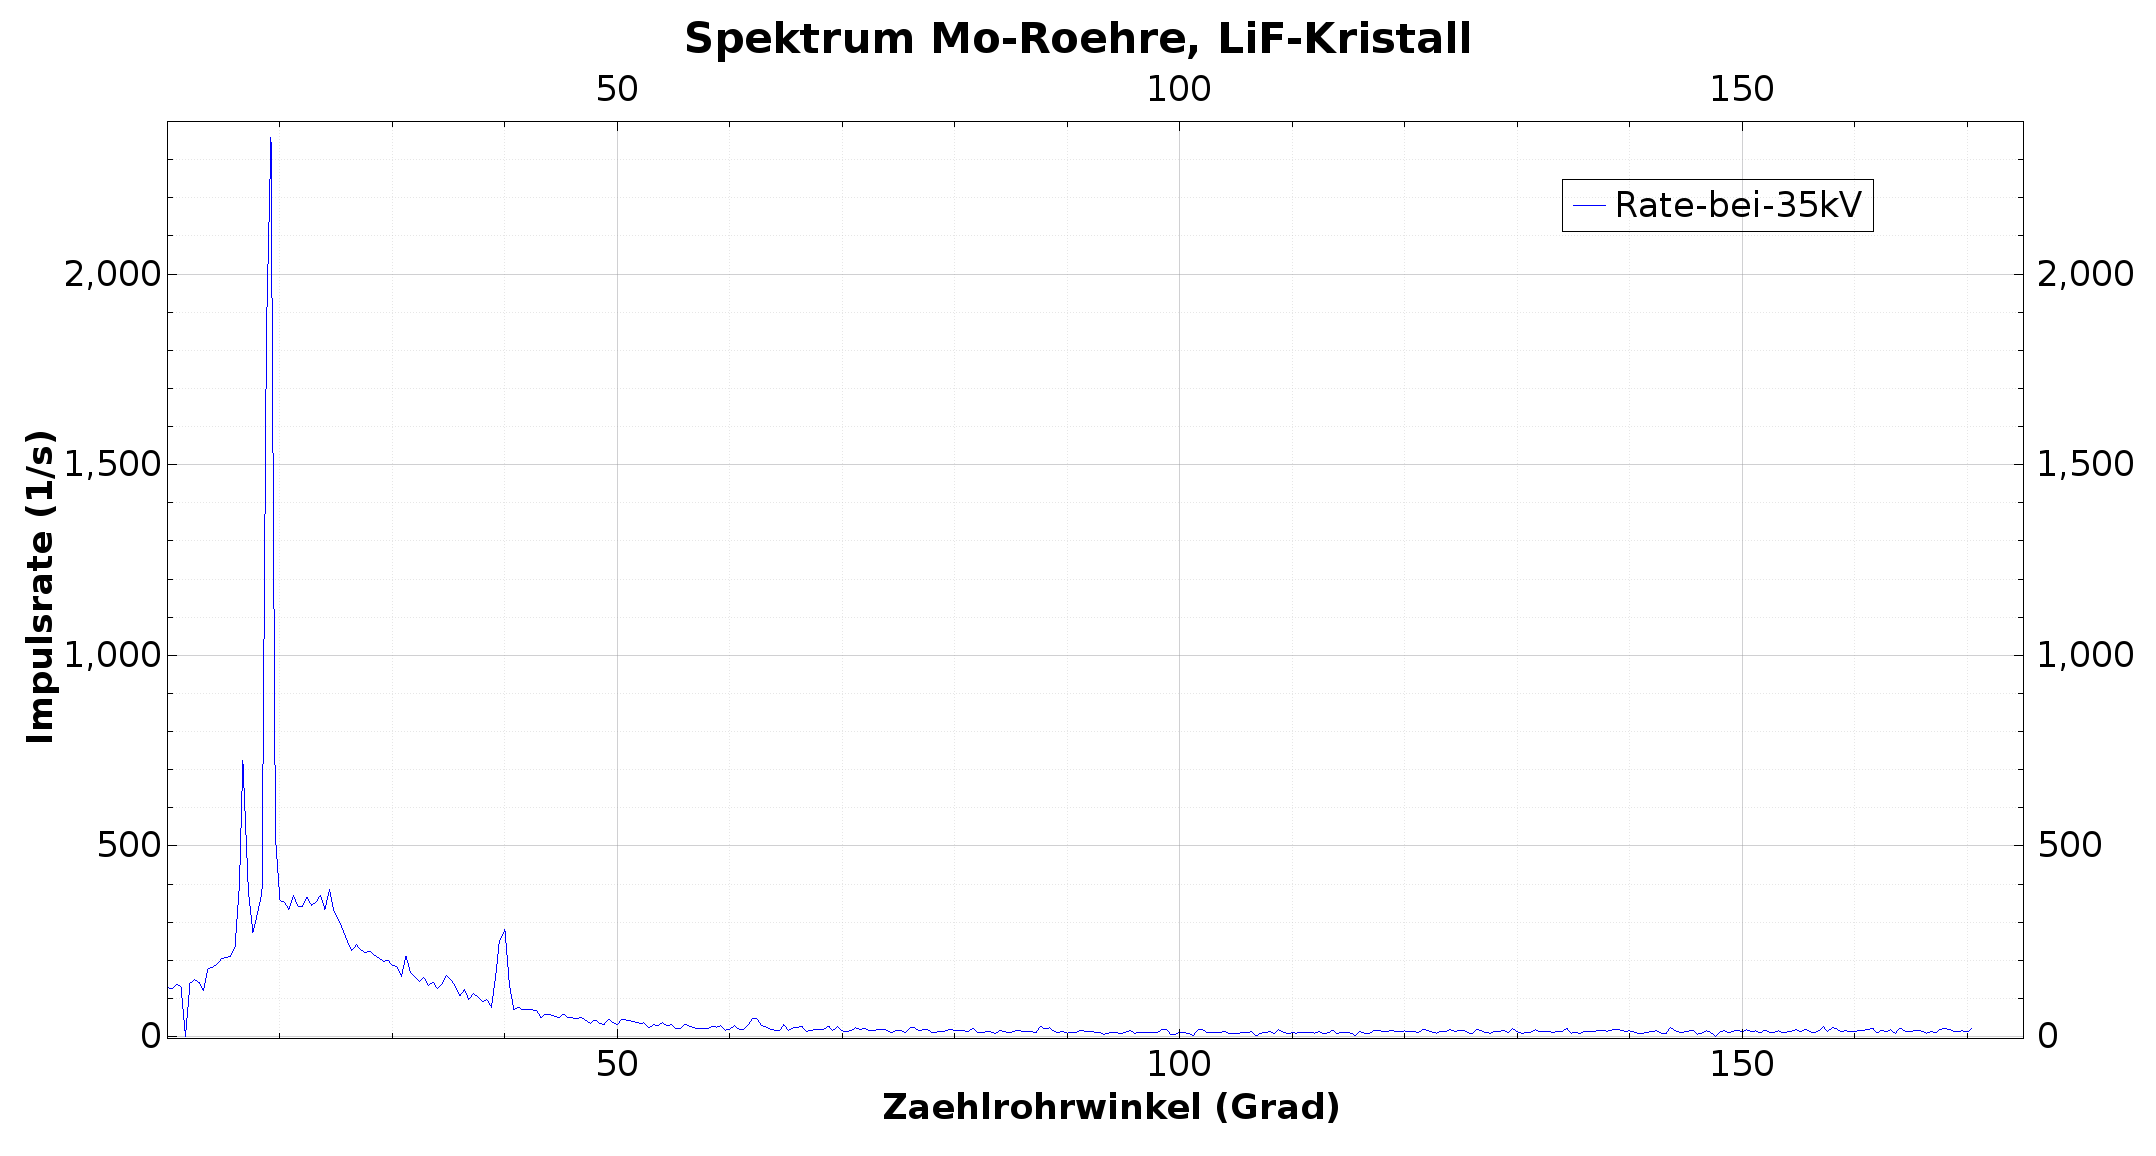
\includegraphics[width=\textwidth]{images/31_3_spektrum-Mo.png}
    \caption{Spektrum mit Molybd\"anr\"ohre}
    \label{fig:spektrum:mo}
\end{figure}

Aus den Daten zu  den Abbildungen \ref{fig:spektrum:cu}, \ref{fig:spektrum:fe}
und \ref{fig:spektrum:mo}  wurden nun die zu  den Spektrallinien geh\"ohrenden
Z\"ahlrohrwinkel  ausgelesen. Dies  erfolgte  \emph{nicht}  aus  dem  Diagramm
direkt, da dies zu ungenau w\"are. Stattdessen wurden dazu die Zahlenwerte der
Messungen mithilfe der Plots (zum Eingrenzen des Suchbereichs) betrachtet.


\begin{table}[h!]
    \centering
    \small
    \caption{%
        Z\"ahlrohrwinkel (entspricht doppeltem  Glanzwinkel) zu Spektrallinien
        mit LiF-Kristall bei \SI{35}{\kilo\volt}
    }
    \label{tab:spektra:LiF}
    \begin{tabular}{lrrrrrr}
        \toprule
        & \multicolumn{2}{l}{Kupferr\"ohre} & \multicolumn{2}{l}{Eisenr\"ohre} & \multicolumn{2}{l}{Molybd\"anr\"ohre} \\
        \midrule

        &
        $2 \cdot \vartheta_\beta$  &
        $2 \cdot \vartheta_\alpha$ &
        $2 \cdot \vartheta_\beta$  &
        $2 \cdot \vartheta_\alpha$ &
        $2 \cdot \vartheta_\beta$  &
        $2 \cdot \vartheta_\alpha$ \\

        \midrule

        n = 1              &
        \SI{39.2}{\degree} &
        \SI{43.6}{\degree} &
        \SI{50.4}{\degree} &
        \SI{56.0}{\degree} &
        \SI{16.7}{\degree} &
        \SI{19.2}{\degree} \\

        n = 2              &
        \SI{ 85.6}{\degree} &
        \SI{ 98.0}{\degree} &
        \SI{120.0}{\degree} &
        \SI{146.8}{\degree} &
        \SI{ 34.8}{\degree} &
        \SI{ 40.0}{\degree} \\

        n = 3              &
                            &
                            &
                            &
        \SI{147.6}{\degree} &
                            &
        \SI{ 62.0}{\degree} \\


        \bottomrule
    \end{tabular}
\end{table}


Schlussendlich  wollen  wir  mit  diesen  Daten  auf  die  Gitterstruktur  des
LiF-Kristalles schliessen. Bevor wir  dies tun, werden wir  jedoch zuerst noch
untersuchen,  ob  sich  allenfalls  ein Nullpunktfehler  in  unsere  Messungen
eingeschlichen hat.

Dazu stellen wir zuerst die Bragg'sche Gleichung um und f\"uhren einen Nullpunktfehler
$\vartheta_0$ ein:

\begin{equation}
    \label{eq:braggNew}
    \vartheta_n = arcsin \left( \frac{n \cdot \lambda_{Anode}}{2 \cdot d} \right) + \vartheta_0
\end{equation}

Als  Stellgr\"osse benutzen  wir nun  $n \cdot  \lambda$, wobei  $\lambda$ aus
Tabelle \ref{tab:anodeSpetralLines}  von Seite \pageref{tab:anodeSpetralLines}
entnommen  wird. Je   nachdem,  ob   es  sich  um   eine  $\beta$-  oder  eine
$\alpha$-Linie handelt, muss nat\"urlich das entsprechende $\lambda$ verwendet
werden.

Dies f\"uhrt zu folgenden Wertepaaren:


\begin{table}[h!]
    \centering
    \small
    \caption{Wertepaare f\"ur umgestellte Bragg'sche Formel}
    \label{tab:anodeSpetralLines}
    \begin{tabular}{rr|rr|rr}
        \toprule

        \multicolumn{2}{l}{Kupfer}     &
        \multicolumn{2}{l}{Eisen}      &
        \multicolumn{2}{l}{Molybd\"an} \\

        \midrule

        $n \cdot \lambda$ &
        $\vartheta_n$     &
        $n \cdot \lambda$ &
        $\vartheta_n$     &
        $n \cdot \lambda$ &
        $\vartheta_n$     \\

        \midrule

        \SI{139.23}{\pico\meter}  & \SI{19.6}{\degree} &
        \SI{175.66}{\pico\meter}  & \SI{25.2}{\degree} &
        \SI{63.26}{\pico\meter}   & \SI{8.35}{\degree} \\

        \SI{154.245}{\pico\meter} & \SI{21.8}{\degree} &
        \SI{193.8}{\pico\meter}   & \SI{28}{\degree} &
        \SI{71.145}{\pico\meter}  & \SI{9.6}{\degree} \\

        \SI{278.46}{\pico\meter}  & \SI{42.8}{\degree} &
        \SI{351.32}{\pico\meter}  & \SI{60}{\degree} &
        \SI{126.52}{\pico\meter}  & \SI{17.4}{\degree} \\

        \SI{308.49}{\pico\meter}  & \SI{49}{\degree} &
        \SI{387.6 }{\pico\meter}  & \SI{73.4}{\degree} &
        \SI{142.29}{\pico\meter}  & \SI{20}{\degree} \\

        & &
        & &
        \SI{213.435}{\pico\meter} & \SI{31}{\degree} \\


        \bottomrule
    \end{tabular}
\end{table}

Nun w\"are es nat\"urlich sehr elegant, wenn man direkt eine Regression \"uber
die  beiden Variablen  $d$ und  $\vartheta_0$ mit  diesen Werten  durchf\"uhren
k\"onnte, und somit  in einem Zug den Netzebenenabstand und  den Offset dieser
Messungen erhielte.

Leider  zeigte  sich  QtiPlot  hierbei aber  sehr  unkooperativ. Trotz  vielem
Herumt\"ufteln  st\"urzte das  Programm beim  Versuch, \"uber  beide Variablen
eine Regression durchzuf\"uhren, ab.

Als Workaround wurde daher folgendermassen vorgegangen:

\begin{itemize}
    \item
        $d$    wurde    auf   den    Wert    aus    der   Literatur    gesetzt
        (\SI{201.5}{\pico\meter}, siehe Versuchsanleitung).
    \item
        Anschliessend  wurde mit  diesem Wert,  der modifizierten  Bragg'scnen
        Formel  aus Gleichung  \ref{eq:braggNew}  und den  Werten aus  Tabelle
        \ref{tab:anodeSpetralLines} eine Regression  durchgef\"uhrt und daraus
        der Nullpunktfehler $\vartheta_0$ bestimmt.
    \item
        Die somit erhaltenen Werte f\"ur den Nullpunktfehler (einer f\"ur jede
        R\"ohre)  wurden anschliessend  mit  Matlab wieder  in die  Bragg'sche
        Formel  aus  \ref{eq:braggNew}  eingesetzt, jedoch  diesmal  nach  dem
        Netzebenenabstand $d$ aufgel\"ost.

        Dabei     erh\"alt     man     f\"ur    jede     Spektrallinie     ein
        Resultat. Diese  k\"onnen  abschliessend noch  gemittelt  werden. Eine
        Fehlerrechnung   wurde  ebenfalls   durchgef\"uhrt  (siehe   Abschnitt
        \ref{subsec:error:spektra} ab Seite \pageref{subsec:error:spektra}).
\end{itemize}

Die   Regressions-Plots  sind   in   den  Abbildungen   \label{fig:offset:cu},
\label{fig:offset:fe} und \label{fig:offset:mo} abgebildet.


\begin{figure}[h!]
    \centering
    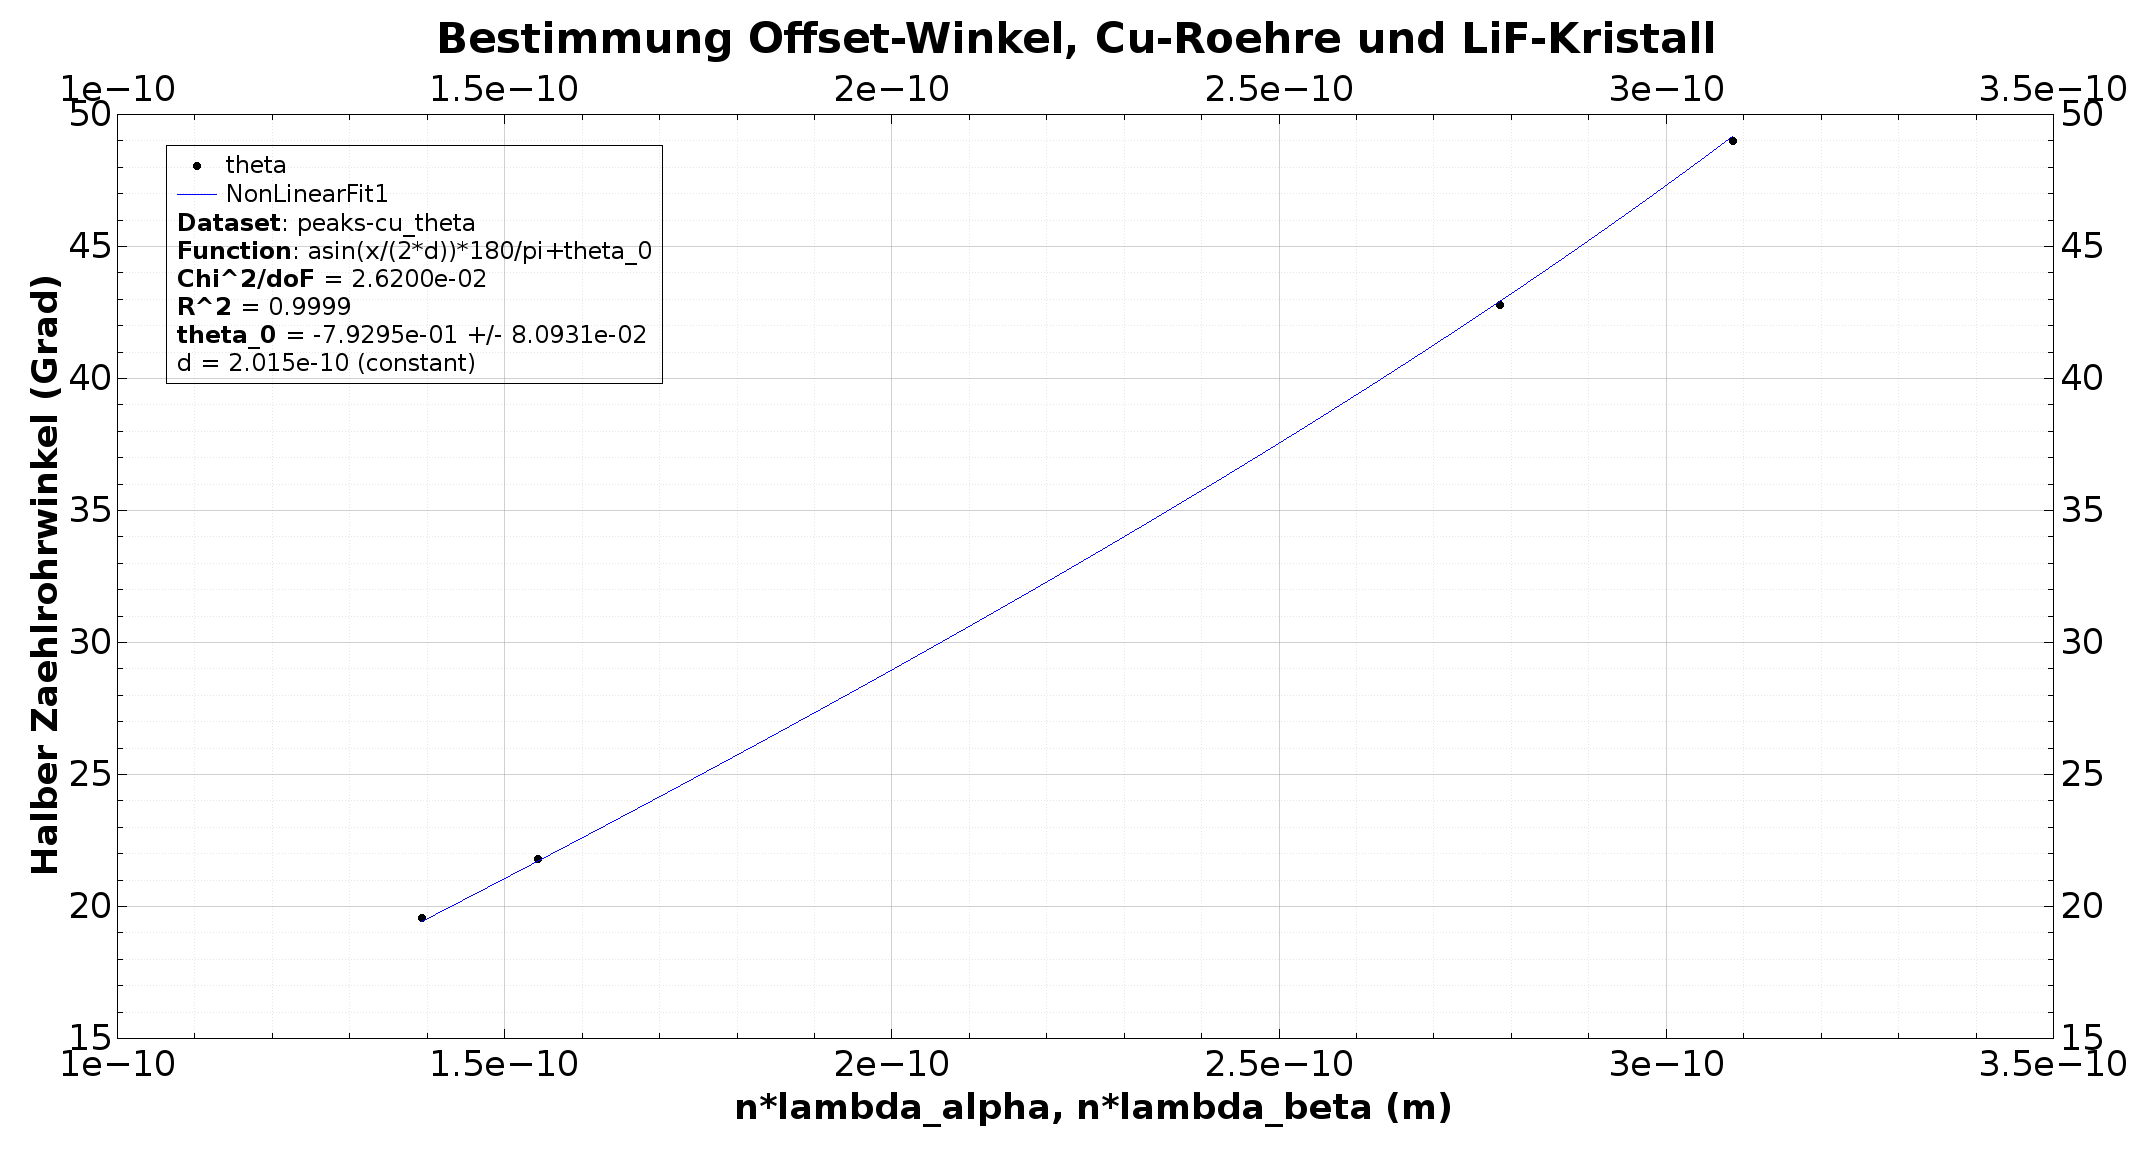
\includegraphics[width=\textwidth]{images/offset-Cu.png}
    \caption{Bestimmung Nullpunktfehler f\"ur Kupferr\"ohre}
    \label{fig:offset:cu}
\end{figure}
Der Nullpunktfehler f\"ur die Messreihe mit der Kupferr\"ohre betr\"agt also:
$$\vartheta_0 = \SI{-0.72925 \pm 0.080931}{\degree}$$

\begin{figure}[h!]
    \centering
    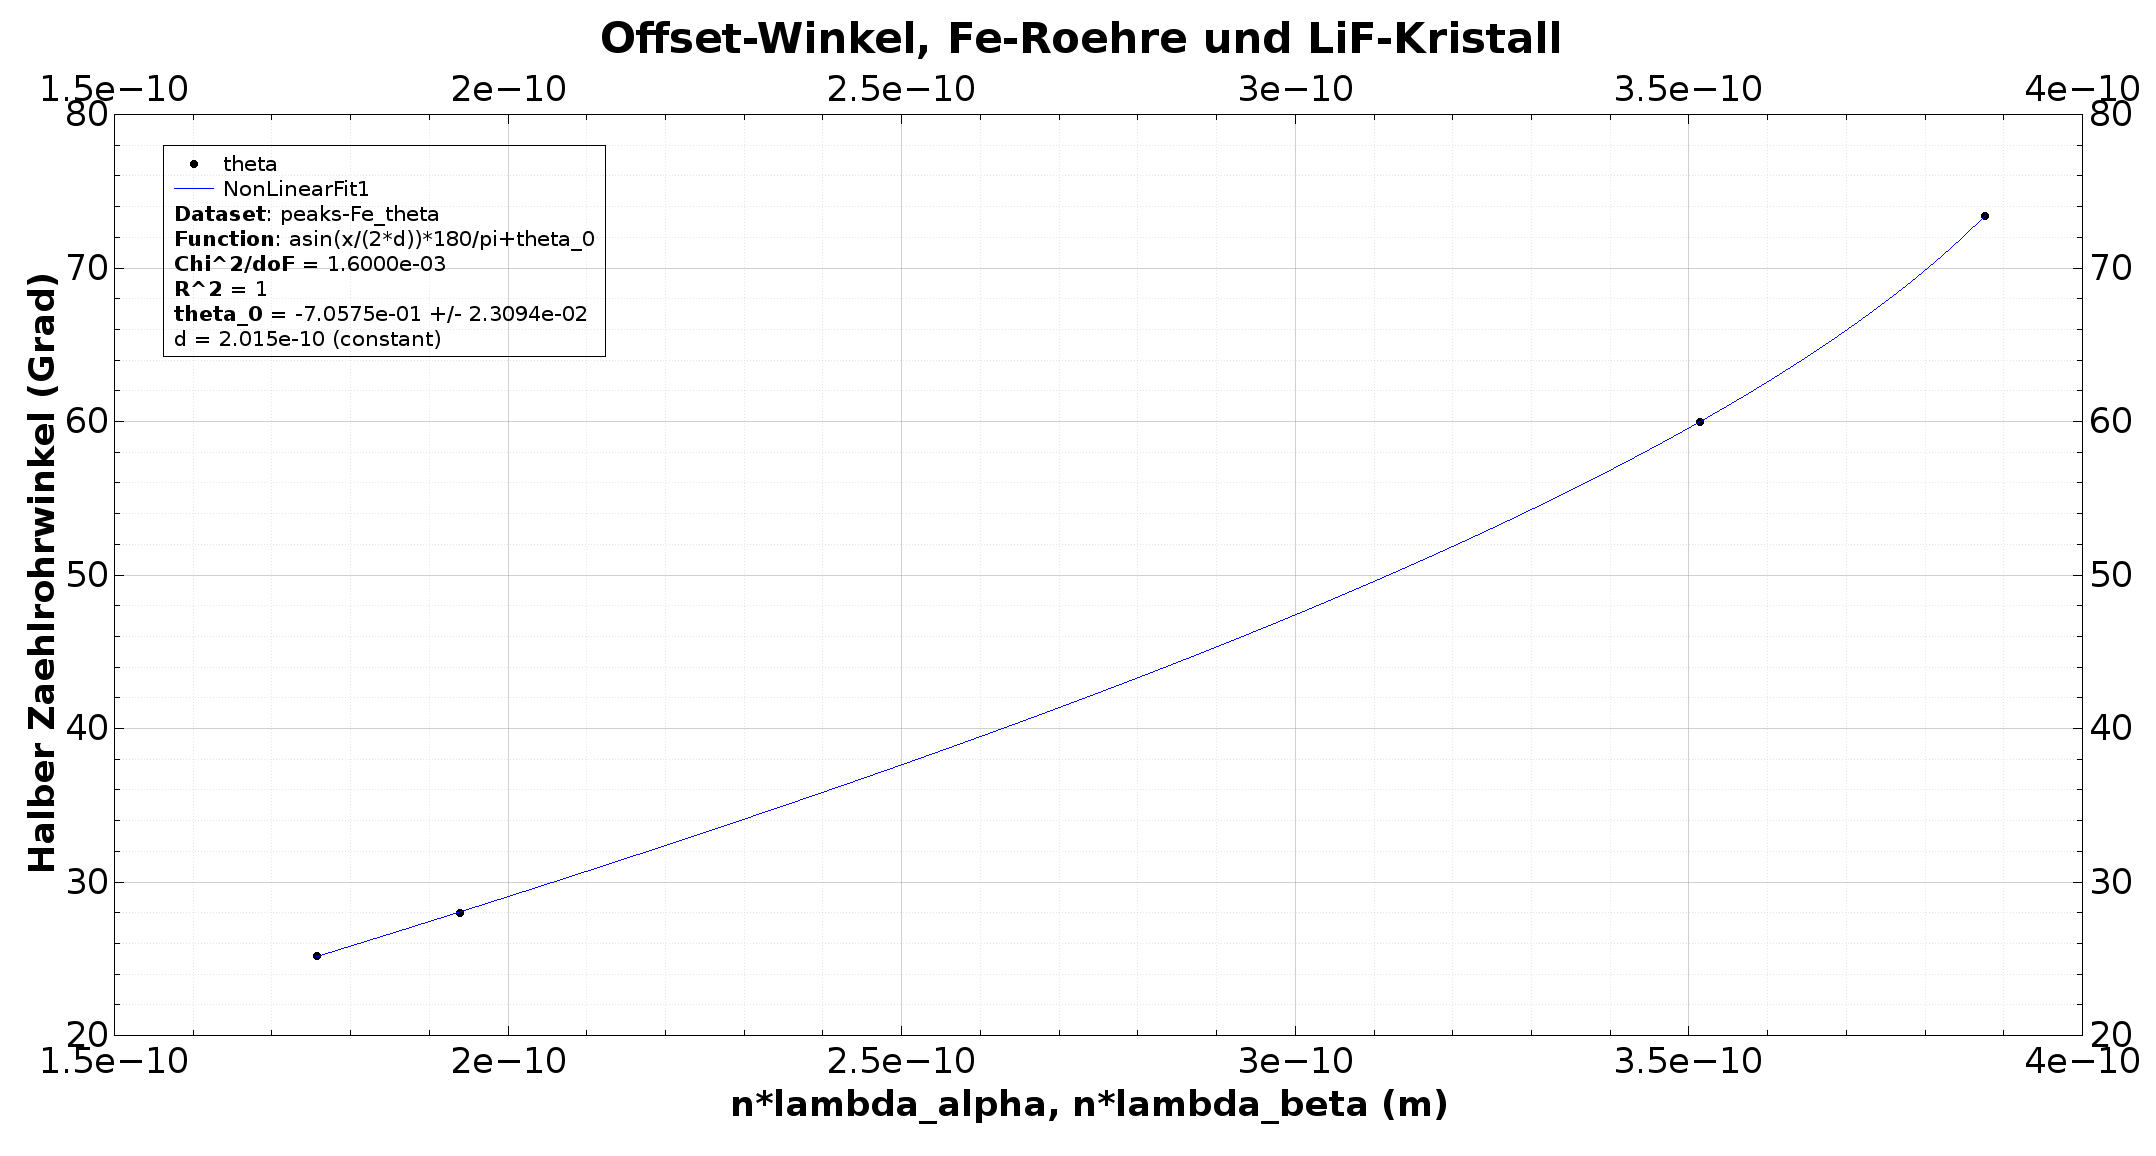
\includegraphics[width=\textwidth]{images/offset-Fe.png}
    \caption{Bestimmung Nullpunktfehler f\"ur Eisenr\"ohre}
    \label{fig:offset:fe}
\end{figure}
Der Nullpunktfehler f\"ur die Messreihe mit der Eisenr\"ohre ist:
$$\vartheta_0 = \SI{-0.70575 \pm 0.023094}{\degree}$$

\begin{figure}[h!]
    \centering
    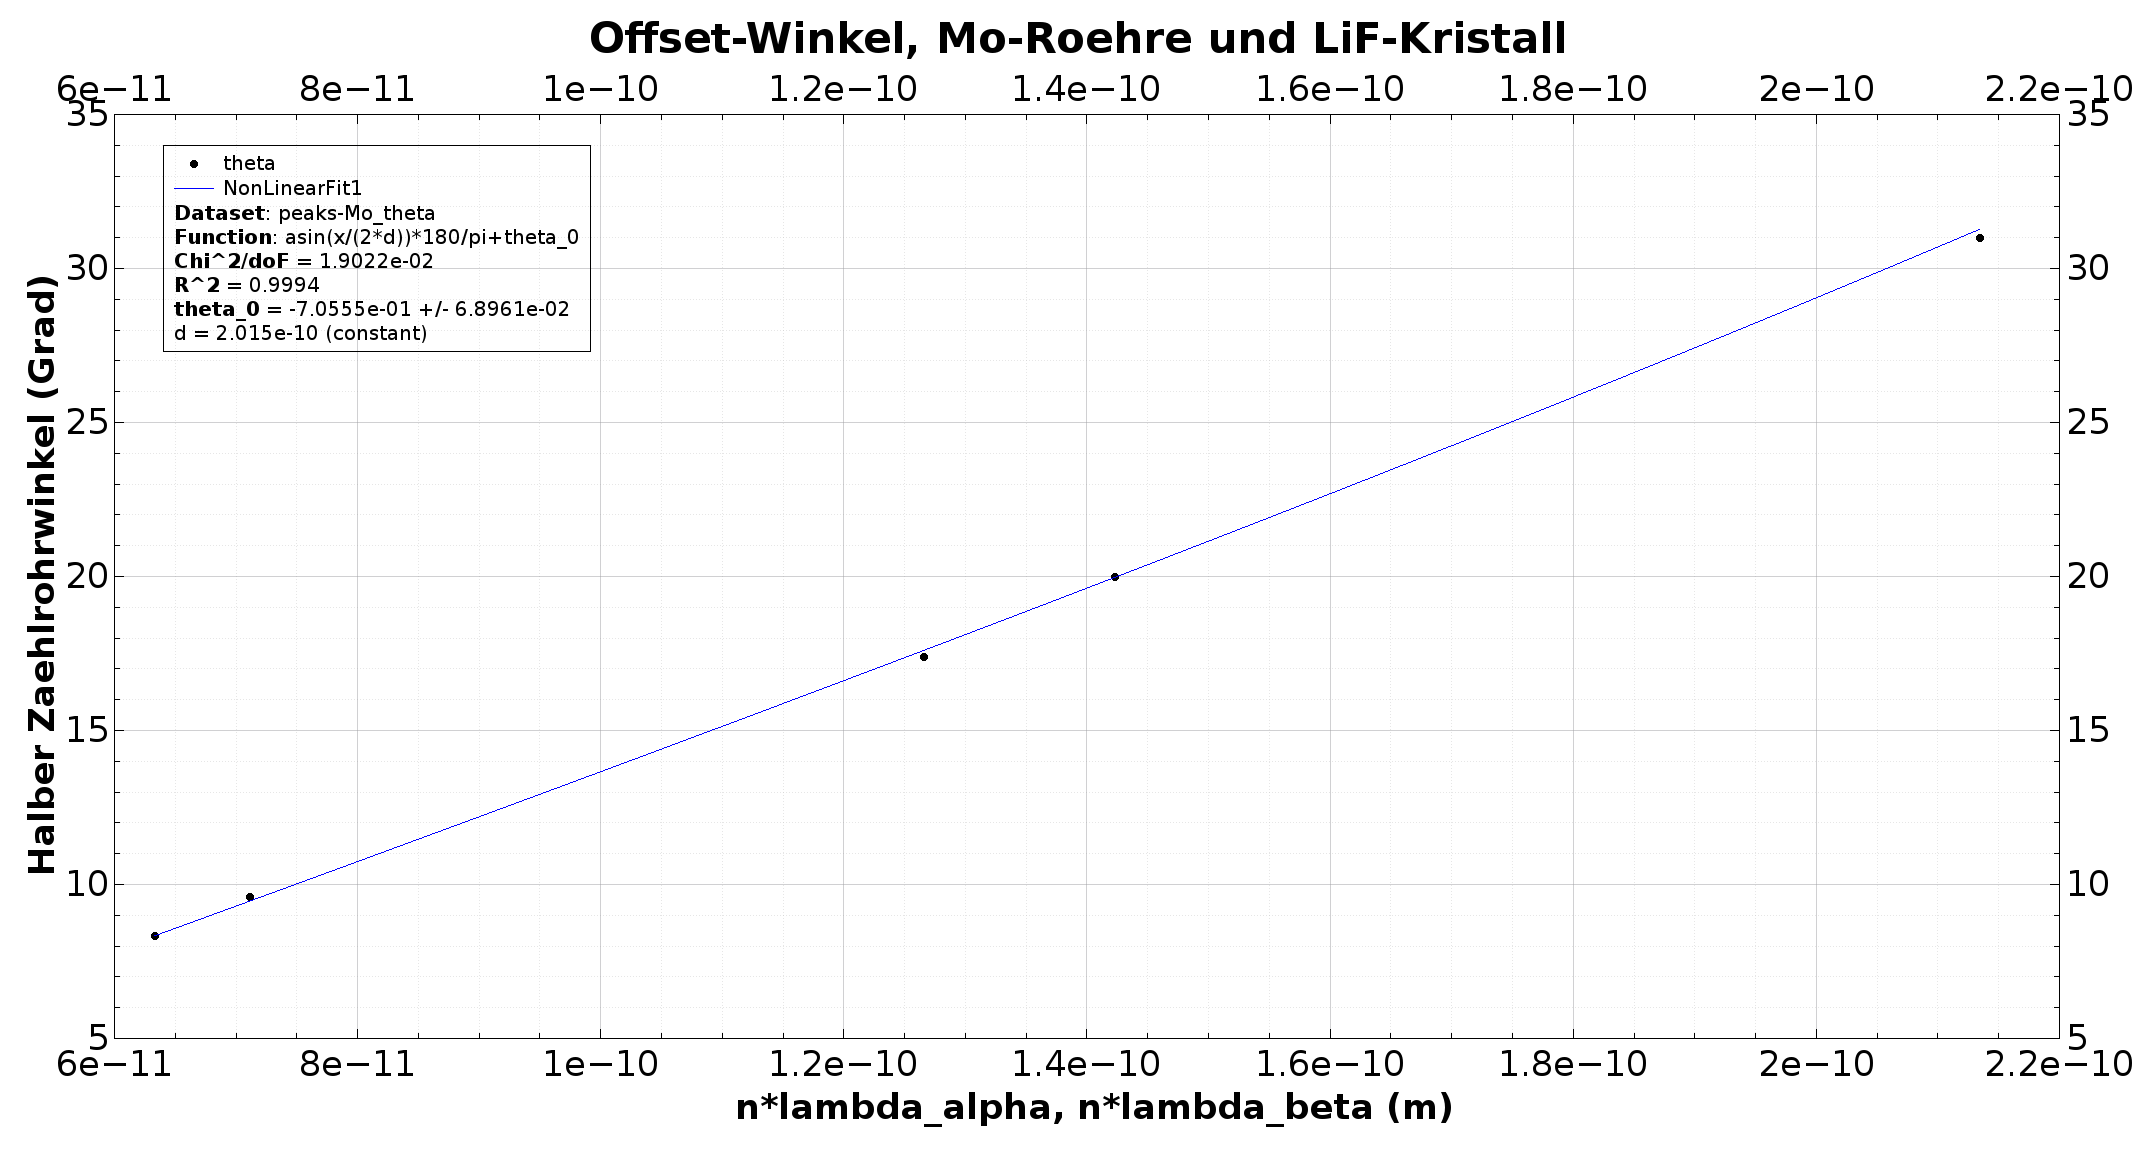
\includegraphics[width=\textwidth]{images/offset-Mo.png}
    \caption{Bestimmung Nullpunktfehler f\"ur Molybd\"anr\"ohre}
    \label{fig:offset:mo}
\end{figure}
Der Nullpunktfehler f\"ur die Messreihe mit der Molybd\"anr\"ohre kommt auf:
$$\vartheta_0 = \SI{-0.70555 \pm 0.068961}{\degree}$$

Die  Weiterverarbeitung dieser  Resultate wurde  inklusive Fehlerrechnung  mit
Matlab durchgef\"uhrt und ist  in Kapitel \ref{subsec:error:spektra} auf Seite
\pageref{subsec:error:spektra} zu finden.

\clearpage
% ---------------------------------------------------------------------------- %
\subsection{Versuch 3.3 -- Planck-Konstante}
\label{subsec:planck}
% ---------------------------------------------------------------------------- %

Das Planck'sche Wirkungsquantum soll \"uber die Grenzwellenl\"ange $\lambda_G$ und
die Formel

\begin{equation*}
    \lambda_G = \frac{h \cdot c}{e \cdot U}
\end{equation*}

bestimmt werden.

Dazu wurden  bei verschiedenen R\"ohrenspannungen Spektren  mit der Fe-R\"ohre
und dem LiF-Kristall aufgenommen, mit besonderem Augenmerk auf den Bereich, wo
$lambda_G$ erwartet wurde (also kleine Z\"ahlrohrwinkel).

Anschliessend  wurden  f\"ur jede  Spannung  der  Scatter-Plot von  Hand  nach
bestem  Wissen  und Gewissen  ausgewertet. Genauer  gesagt  wurde eine  Gerade
m\"oglichst sinnvoll durch die Messpunkte gelegt und ihre Schnittpunkt mit der
horizontalen Achse bestimmt, inklusive abgesch\"atzter Unsicherheit.

Eine   schematische   Darstellung   dieses    Prozesses   ist   in   Abbildung
\ref{fig:planckDemo} auf Seite \pageref{fig:planckDemo} zu sehen.

Die bestimmten  Werte wurden  anschliessend in ein  Matlab-Script gef\"uttert,
welches  daraus  die   zugeh\"origen  Grenzwellenl\"angen  und  Unsicherheiten
berechnete.

Dem  aufmerksamen  Leser  wird  auffallen, dass  eine  Mess-Serie  fehlt. Dies
ist  auf  einen  Fehler  beim  Speichern  der  Daten  zur\"uckzuf\"uhren;  der
Experimentator \"uberschrieb versehentlich ein  Datenset. Dies soll uns jedoch
nicht daran  hindern, diese Auswertung wie  geplant weiterzuf\"uhren. Wie sich
zeigen wird, ist das Resultat trotzdem ganz passabel.

\begin{sidewaysfigure}[h!]
    \centering
    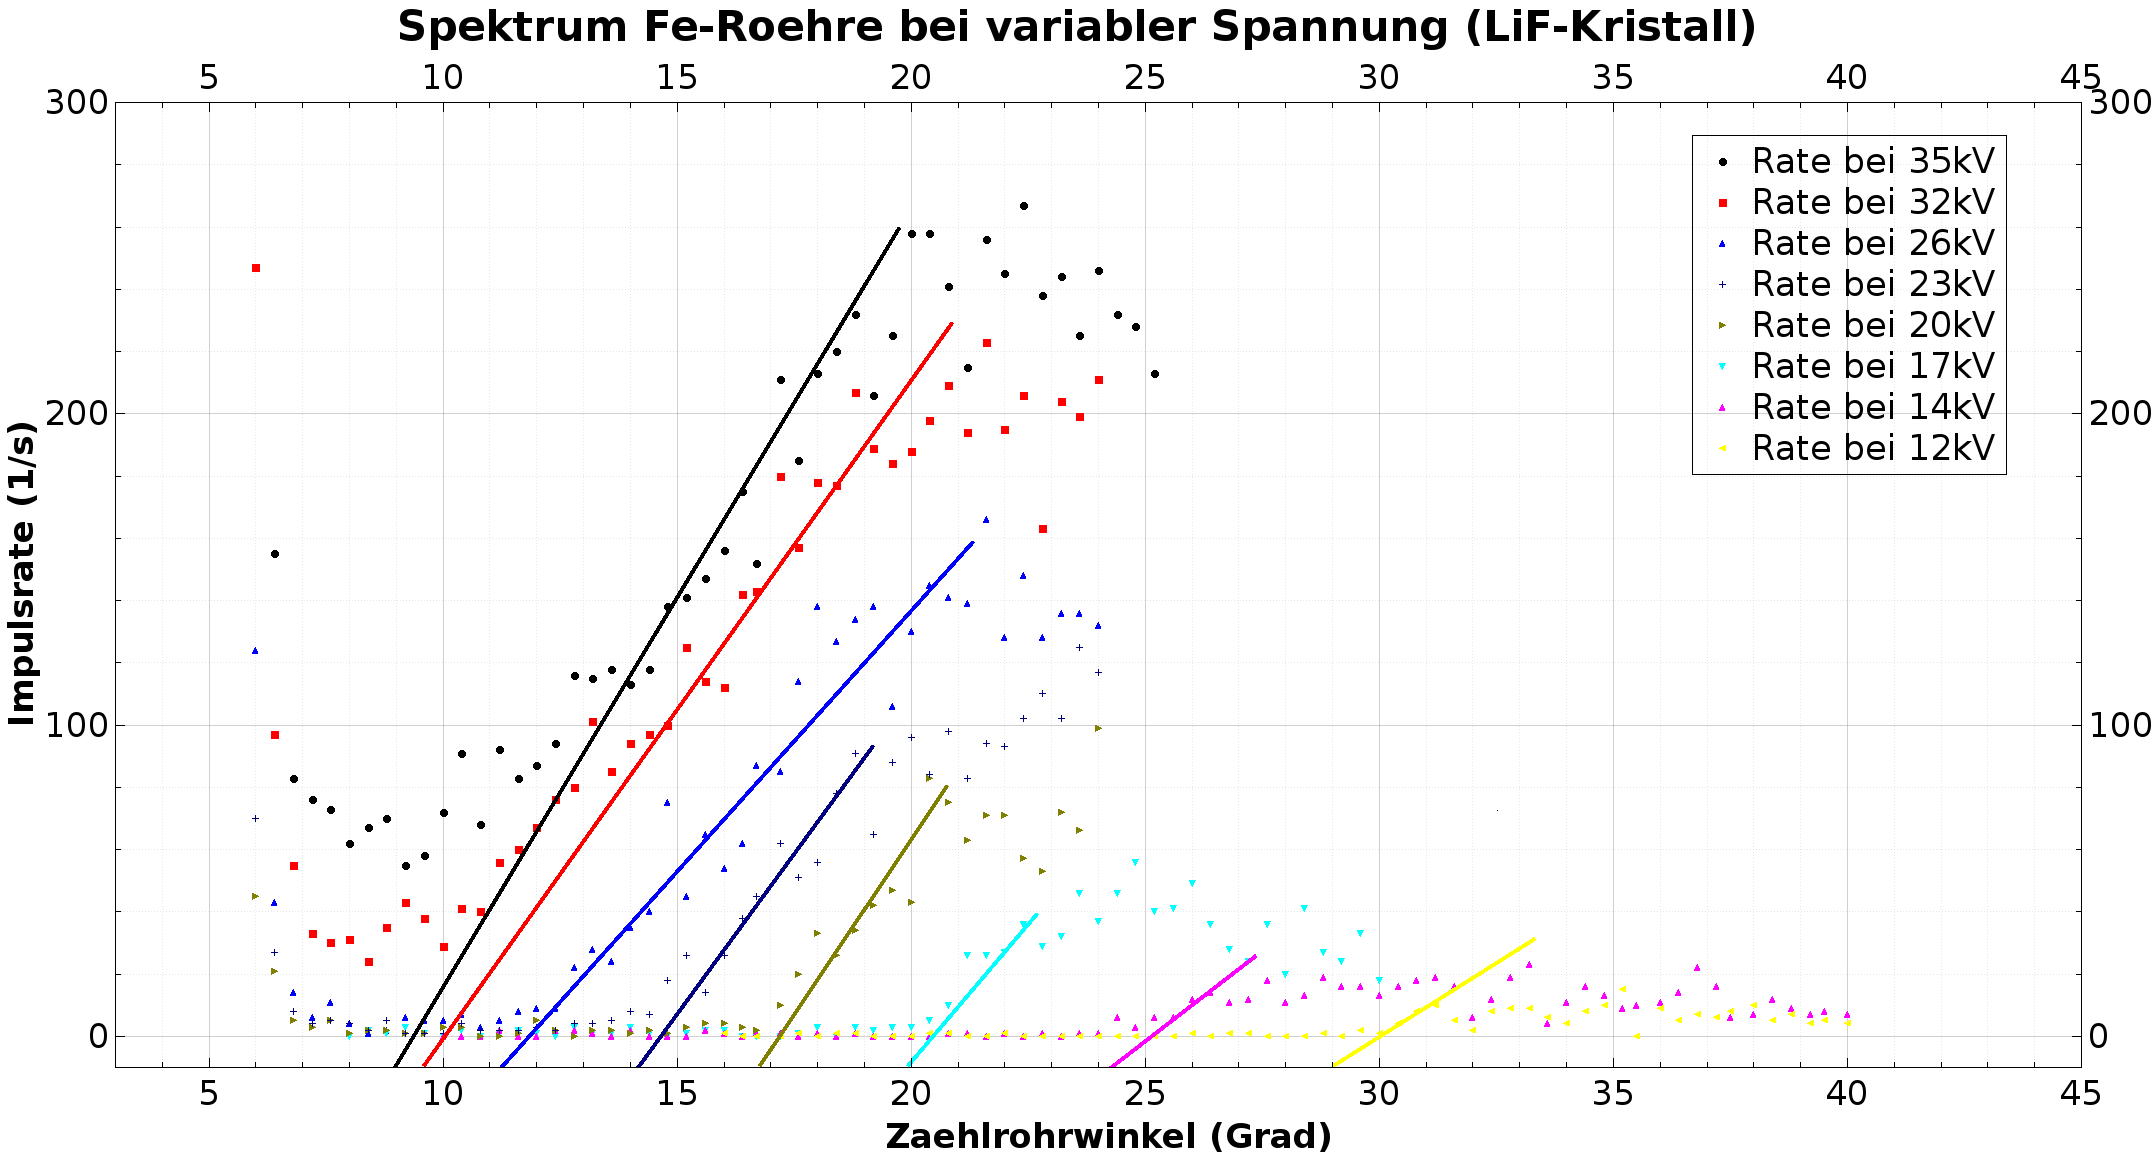
\includegraphics[width=\textwidth]{images/33_0.png}
    \caption{%
        Schematische    Darstellung    der   Bestimmung    der    Grenzwinkel.
        \textbf{Beachte:} Die     hier     eingezeichneten    Geraden     sind
        nicht     diejenigen,     welche     wirklich    zu     den     Werten
        aus     Tabelle     \ref{tab:resultsPlanckManualFit}     auf     Seite
        \pageref{tab:resultsPlanckManualFit}  gef\"uhrt haben. Dazu  ist diese
        Grafik viel  zu grob. Es  wurde pro  Spannung jeweils  ein Scatterplot
        ausgewertet, um  die zugeh\"origen  Grenzwinkel zu  bestimmen. Da dies
        jedoch  unverh\"altnism\"assig  viel  Platz  ben\"otigt  f\"ur  diesen
        Bericht, ist das Vorgehen schematisch hier dargestellt.
    }
    \label{fig:planckDemo}
\end{sidewaysfigure}

\begin{table}[h!]
    \centering
    \small
    \caption{Grenzwinkel $\vartheta_G$ und Grenzwellenl\"ange $\lambda_G$}
    \label{tab:resultsPlanckManualFit}
    \begin{tabular}{rrr}
        \toprule
        Spannung U          & Winkel $2 \cdot \vartheta_G$      & Wellenl\"ange (Matlab) \\
        \midrule
        \SI{35}{\kilo\volt} &       \SI{9     \pm~1.5}{\degree} & \SI{ 36.62 \pm 5  }{\pico\meter} \\
        \SI{32}{\kilo\volt} &       \SI{9.8   \pm~0.5}{\degree} & \SI{ 39.42 \pm 2  }{\pico\meter} \\
        \SI{26}{\kilo\volt} &       \SI{11.5  \pm~2.5}{\degree} & \SI{ 45.37 \pm 9  }{\pico\meter} \\
        \SI{23}{\kilo\volt} &       \SI{14.2  \pm~0.5}{\degree} & \SI{ 54.79 \pm 2  }{\pico\meter} \\
        \SI{20}{\kilo\volt} &       \SI{16.9  \pm~0.1}{\degree} & \SI{ 64.18 \pm 0.4}{\pico\meter} \\
        \SI{17}{\kilo\volt} &       \SI{20.1  \pm~0.1}{\degree} & \SI{ 75.26 \pm 0.4}{\pico\meter} \\
        \SI{14}{\kilo\volt} &       \SI{24.5  \pm~0.7}{\degree} & \SI{ 90.41 \pm 2  }{\pico\meter} \\
        \SI{12}{\kilo\volt} &       \SI{28.9  \pm~0.5}{\degree} & \SI{105.41 \pm 2  }{\pico\meter} \\
        \bottomrule
    \end{tabular}
\end{table}

Die Wellenl\"angen  aus Tabelle \ref{tab:resultsPlanckManualFit}  wurden dabei
mittels  der  Bragg'schen Gleichung  berechnet,  wobei  $n  =  1$ sowie  $d  =
\SI{201.5}{\pico\meter}$ zu setzen sind.

Die so ermittelten Wellenl\"angen und ihre Fehler wurden nun in QtiPlot eingegeben
und eine gewichtete Regression ausgef\"uhrt.

\begin{figure}[h!]
    \centering
    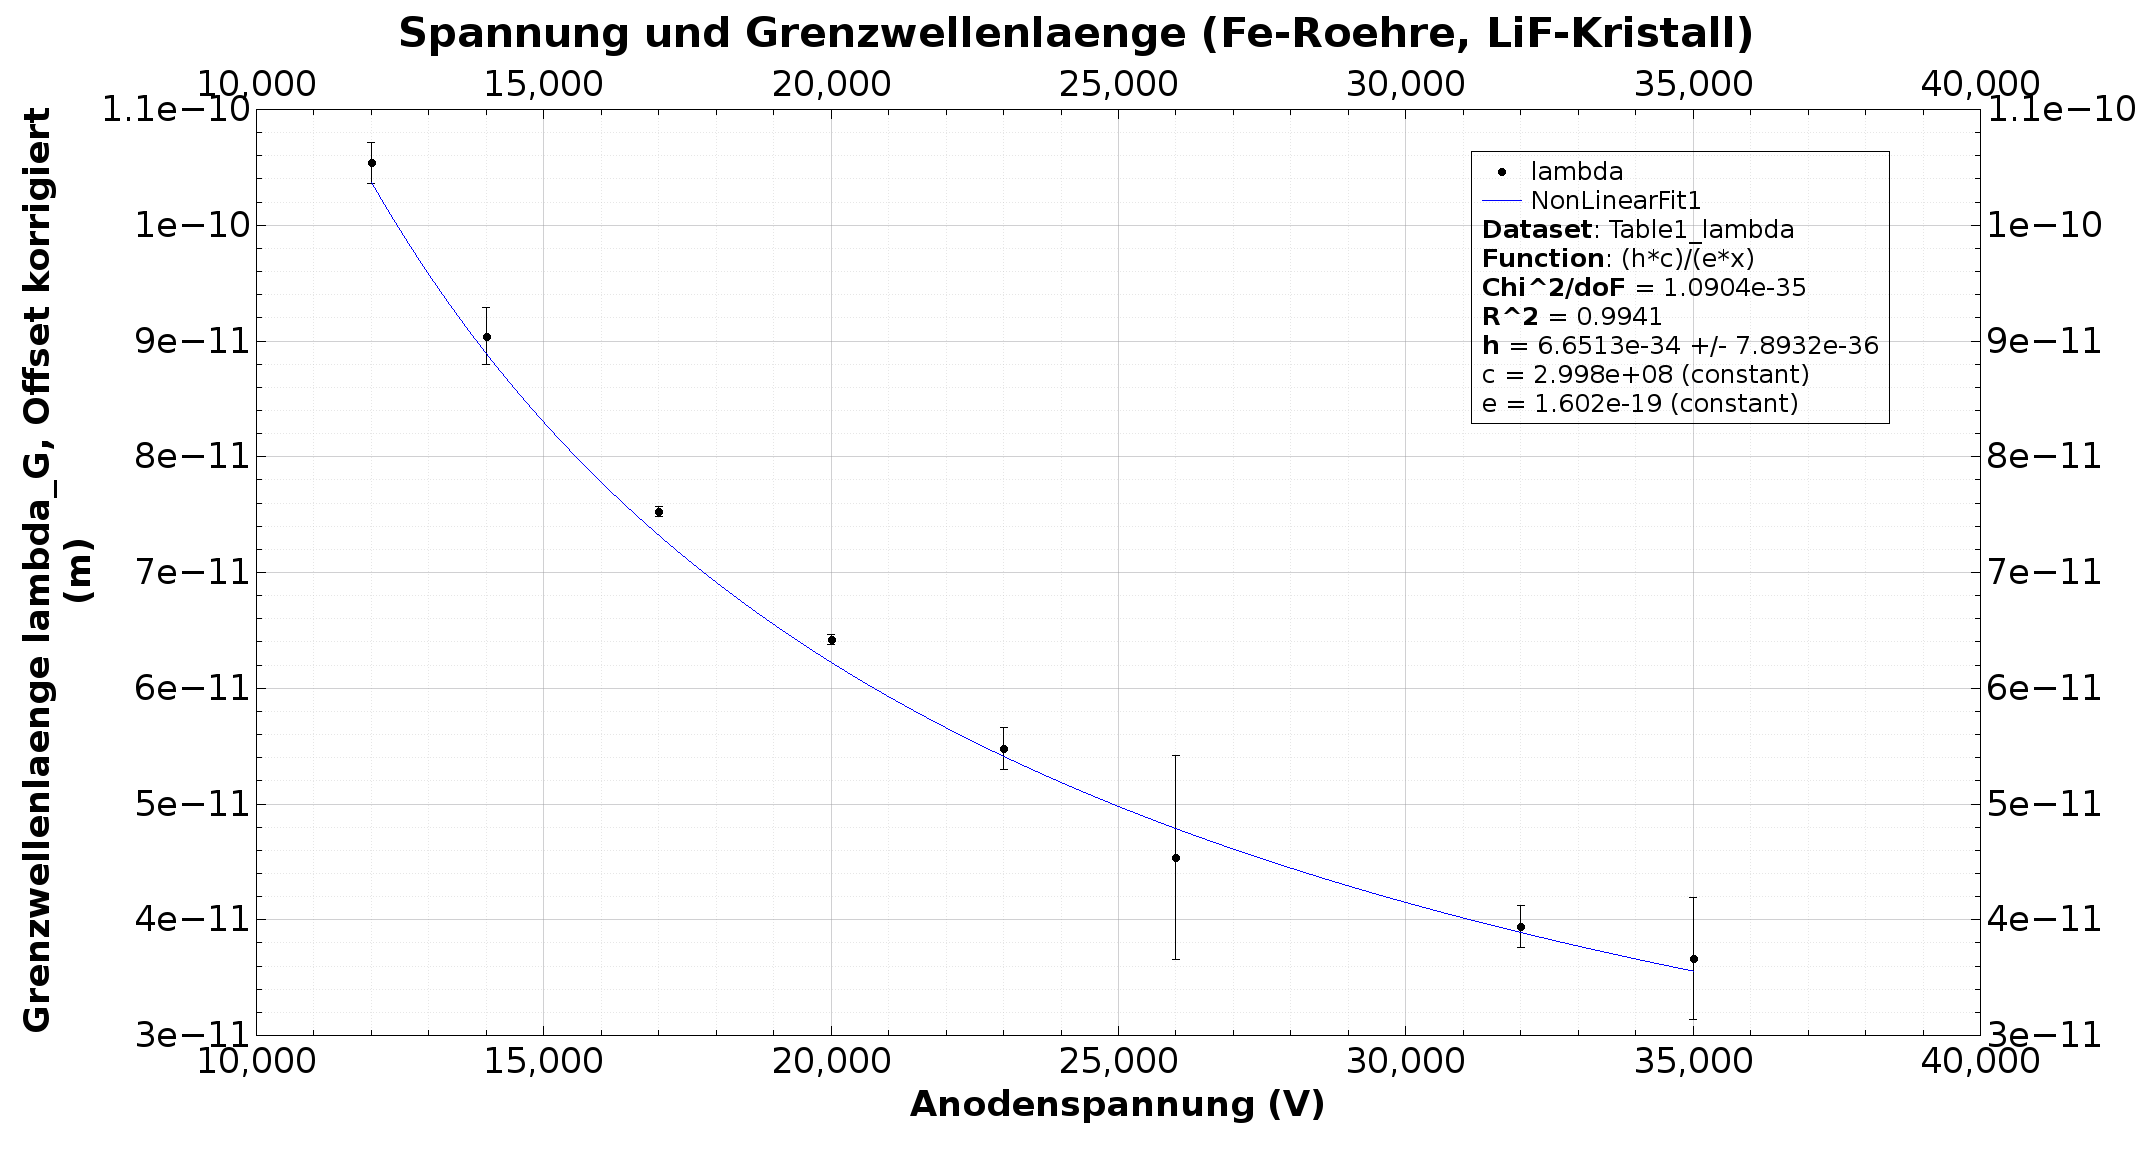
\includegraphics[width=\textwidth]{images/planck.png}
    \caption{Gewichtete Regression zur Bestimmung der Planck'schen Konstante}
    \label{fig:planck}
\end{figure}

\begin{equation*}
    h = \SI{6.6513 \pm 0.08}{\joule\second} \cdot 1e-34
\end{equation*}

\clearpage
% ---------------------------------------------------------------------------- %
\subsection{Andere Kristalle}
\label{subsec:othercrystals}
% ---------------------------------------------------------------------------- %

Hier  ging  es darum,  die  Netzebenenabst\"ande  von diversen  Kristallproben
analog  zum  Abschnitt   \ref{subsec:spektra}  zu  bestimmen. Die  verwendeten
Kristalle waren:

\begin{itemize}
    \item
        Bergkristall (SiO)
    \item
        Kalkspat (Kalzit, CaCO3)
    \item
        Pyrit (Katzengold, FeS2)
    \item
        synthetischer Quartz (SiO2)
\end{itemize}

Hierzu    wurde    von   jedem    Kristall    mit    der   Eisenr\"ohre    bei
\SI{35}{\kilo\volt}  ein   Spektrum  aufgenommen. Diese   sind  zu   sehen  in
den Abbildungen  \ref{fig:spektrum:bergkristall}, \ref{fig:spektrum:kalkspat},
\ref{fig:spektrum:pyrit} und \ref{fig:spektrum:synth_quartz}, die ausgelesenen
Z\"ahlrohrwinkel  sind in  Tabelle  \ref{tab:spektra:otherCrystals} auf  Seite
\pageref{tab:spektra:otherCrystals} zu finden.

\begin{figure}[h!]
    \centering
    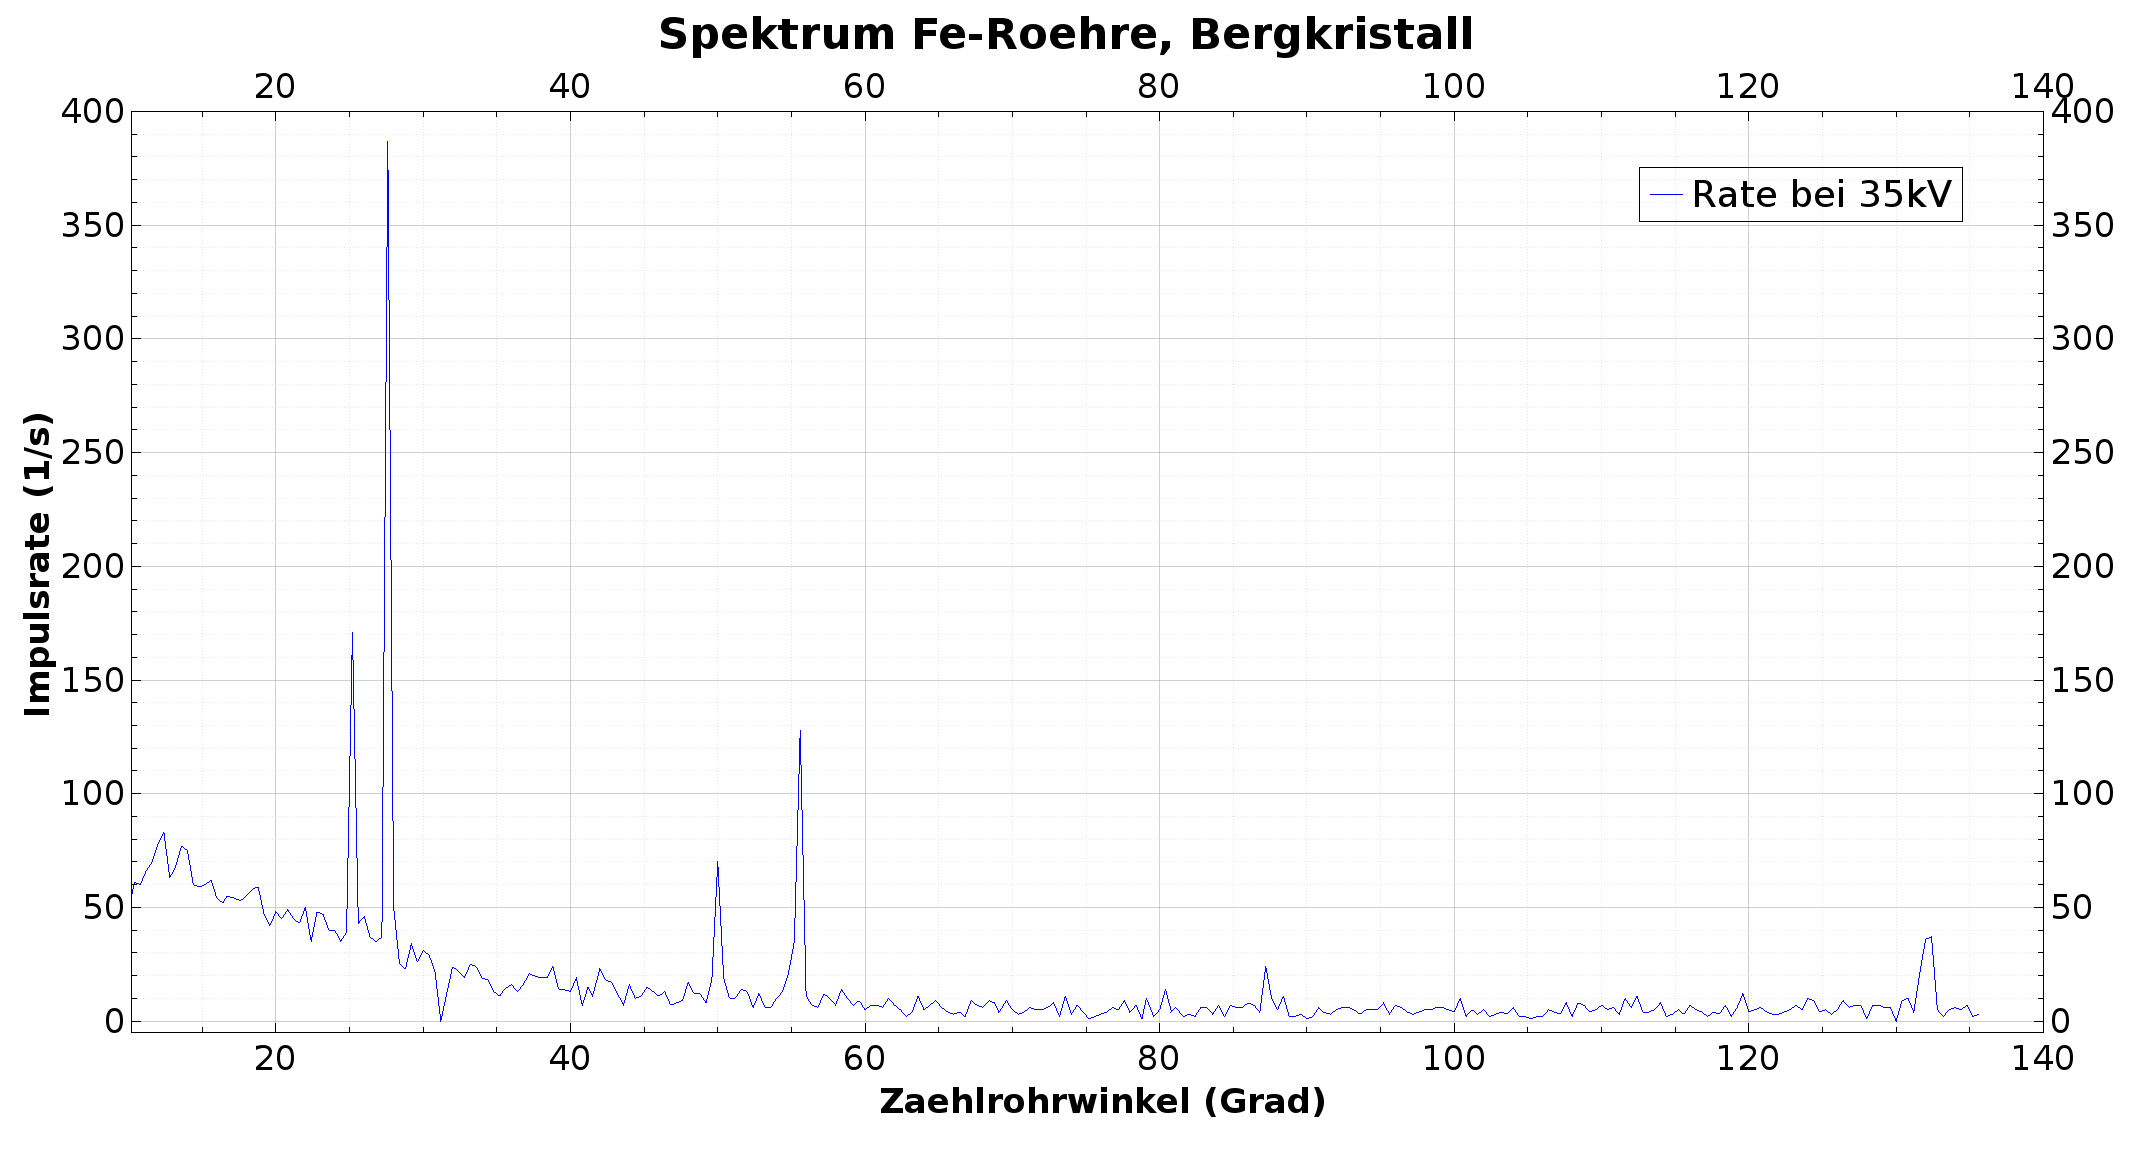
\includegraphics[width=\textwidth]{images/bergkristall-spektrum.png}
    \caption{Spektrum des Bergkristalls mit Eisenr\"ohre bei \SI{35}{\kilo\volt}}
    \label{fig:spektrum:bergkristall}
\end{figure}

\begin{figure}[h!]
    \centering
    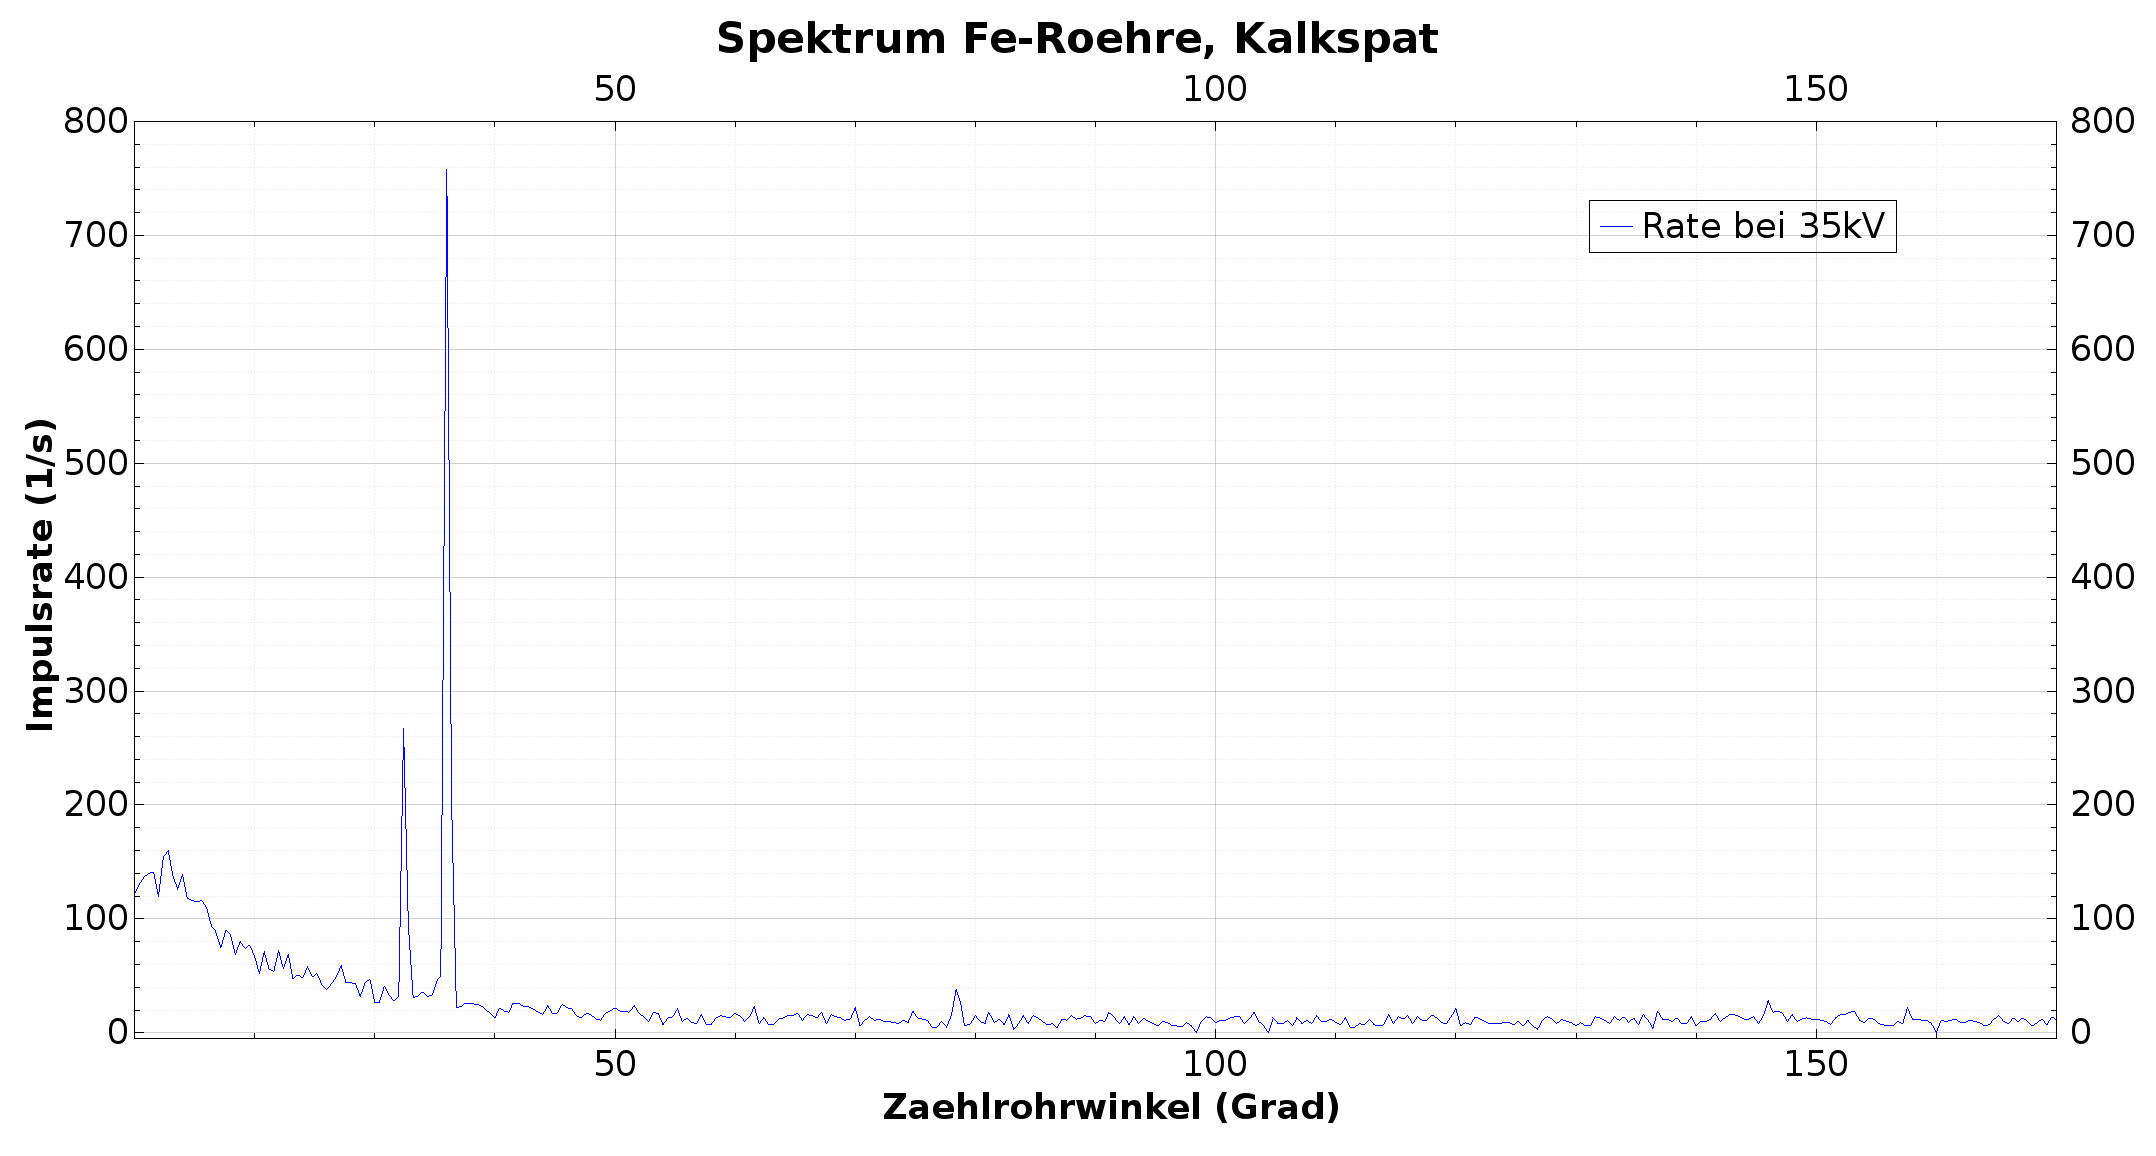
\includegraphics[width=\textwidth]{images/kalkspat-spektrum.png}
    \caption{Spektrum von Kalkspat  mit Eisenr\"ohre bei \SI{35}{\kilo\volt}}
    \label{fig:spektrum:kalkspat}
\end{figure}

\begin{figure}[h!]
    \centering
    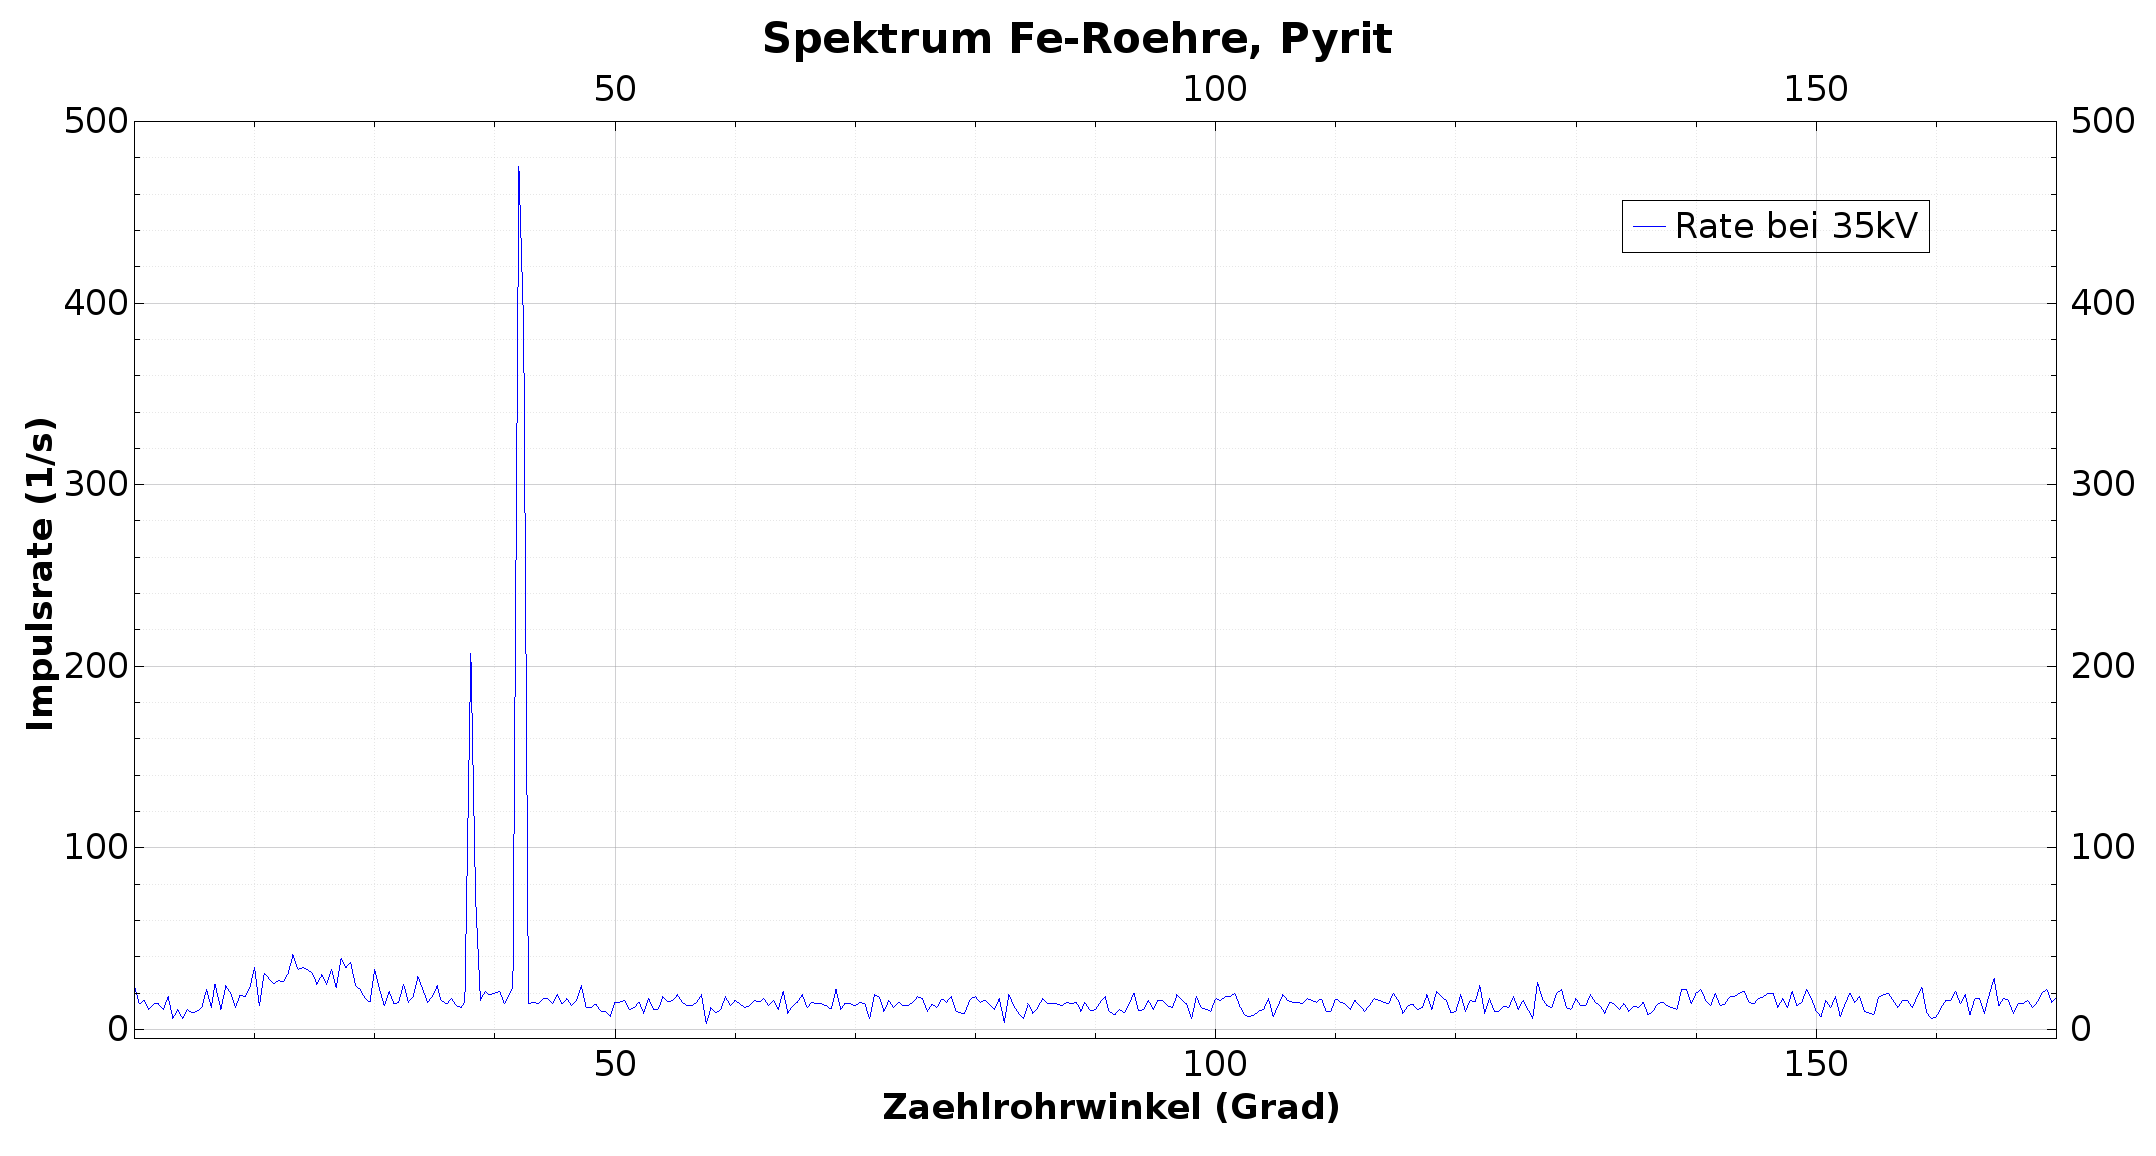
\includegraphics[width=\textwidth]{images/pyrit-spektrum.png}
    \caption{Spektrum von Pyrit  mit Eisenr\"ohre bei \SI{35}{\kilo\volt}}
    \label{fig:spektrum:pyrit}
\end{figure}

\begin{figure}[h!]
    \centering
    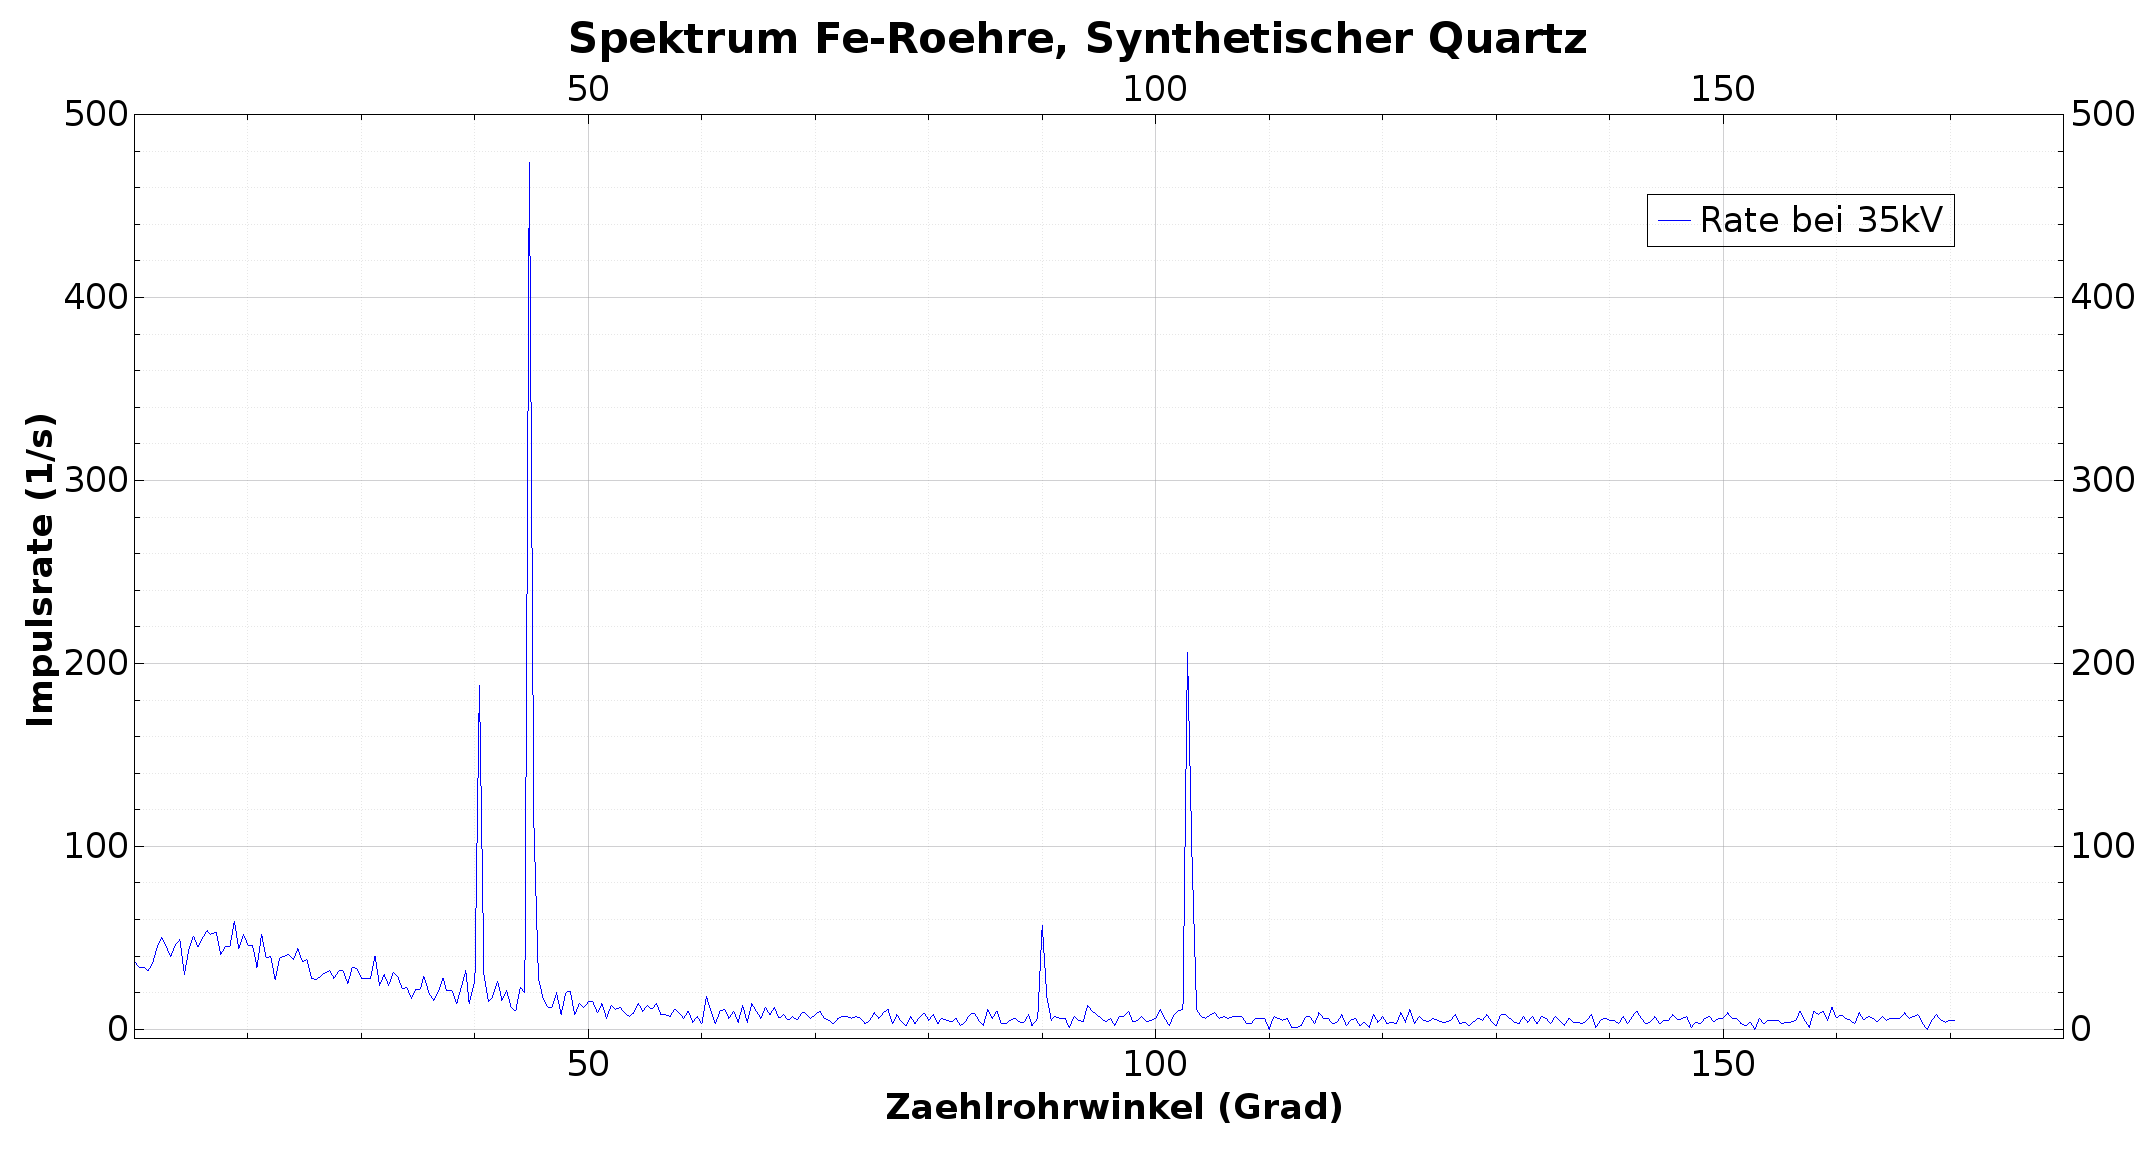
\includegraphics[width=\textwidth]{images/synth-quartz-spektrum.png}
    \caption{Spektrum von synthetischem Quartz  mit Eisenr\"ohre bei \SI{35}{\kilo\volt}}
    \label{fig:spektrum:synth_quartz}
\end{figure}

\begin{table}[h!]
    \centering
    \small
    \caption{%
        Z\"ahlrohrwinkel (entspricht doppeltem  Glanzwinkel) zu Spektrallinien
        mit Fe-R\"ohre bei \SI{35}{\kilo\volt}
    }
    \label{tab:spektra:otherCrystals}
    \begin{tabular}{lrrrrrrrr}
        \toprule
        &
        \multicolumn{2}{l}{Bergkristall}         &
        \multicolumn{2}{l}{Kalkspat}             &
        \multicolumn{2}{l}{Pyrit}                &
        \multicolumn{2}{l}{Synthetischer Quartz} \\
        \midrule

        &
        $2 \cdot \vartheta_\beta$  &
        $2 \cdot \vartheta_\alpha$ &
        $2 \cdot \vartheta_\beta$  &
        $2 \cdot \vartheta_\alpha$ &
        $2 \cdot \vartheta_\beta$  &
        $2 \cdot \vartheta_\alpha$ &
        $2 \cdot \vartheta_\beta$  &
        $2 \cdot \vartheta_\alpha$ \\

        \midrule

        n = 1              &
        \SI{25.2}{\degree} &
        \SI{27.6}{\degree} &
        \SI{32.4}{\degree} &
        \SI{36.0}{\degree} &
        \SI{38.0}{\degree} &
        \SI{42.0}{\degree} &
        \SI{40.4}{\degree} &
        \SI{44.8}{\degree} \\

        n = 2               &
        \SI{ 50.0}{\degree} &
        \SI{ 55.6}{\degree} &
        \SI{ 74.8}{\degree} &
        \SI{ 78.4}{\degree} &
                            &
                            &
        \SI{ 90.0}{\degree} &
        \SI{102.8}{\degree} \\

        n = 3               &
        \SI{ 80.4}{\degree} &
        \SI{ 87.2}{\degree} &
                            &
                            &
                            &
                            &
                            &
                            \\

        n = 4               &
        \SI{119.6}{\degree} &
        \SI{132.4}{\degree} &
                            &
                            &
                            &
                            &
                            &
                            \\

        \bottomrule
    \end{tabular}
\end{table}

Wie  bereits bei  der  Bestimmung des  Netzebenenabstandes des  LiF-Kristalles
erw\"ahnt,  w\"are es  nat\"urlich  sehr elegant  gewesen,  mit diesen  Werten
nun  eine  Regression \"uber  den  Netzebenenabstand  und den  Nullpunktfehler
durchzuf\"uhren. Da   das  (vergebliche)   Debuggen   von   QtiPlot  und   das
Heraust\"ufteln des im Abschnitt  zum LiF-Kristall benutzten Workarounds sowie
seine anschliessende  Umsetzung betr\"achtlich Zeit  in Anspruch nahm,  war es
nicht  mehr  m\"oglich,  diesen  Workaround  auch  auf  diese  vier  Kristalle
anzuwenden.

Die  etwas unelegantere  Methode  besteht  darin, zu  jedem  Wert aus  Tabelle
\ref{tab:spektra:otherCrystals}  den  zugeh\"origen Netzebenenabstand  mittels
der Bragg'schen Gleichung  zu bestimmen, und diese  Resultate anschliessend zu
mitteln. Dieser  Weg  wurde  f\"ur  diesen  Abschnitt  gew\"ahlt  und  ist  im
Kapitel  zur  Fehlerberechnung ab  Seite  \pageref{subsec:error:othercrystals}
beschrieben. Das   Verfahren   wurde   wie  beim   LiF-Kristall   mit   Matlab
ausgef\"uhrt.
